\chapter{Methodik}
\label{chap:methodik}

Für die Segmentierung der Marsoberfläche wird der Ansatz von Kanezaki \etal \cite{kanezaki_18} aus Unterabschnit~\ref{ssec:kanezaki} abgewandelt. Das Ziel besteht daraus, eine Eingabebilddatei durch neuronale Netze zu segmentieren, ohne vorhandene Ground Truth.

Zur Modifikation des genannten Algorithmus existieren viele unterschiedliche Möglichkeiten, einzelne Elemente zu ersetzen, welche in den folgenden Abschnitten beschrieben werden. Nachdem kurz auf die gesamte Funktionsweise des Algorithmus eingegangen wird folgt eine Übersicht über den Initialisierungsalgorithmus und Wege, diesen zu Optimieren. Dazu zählen \bspw unterschiedliche Filterbänke, deren Größen, Gewichtungen der Merkmale und Anzahl der zu generierenden Cluster. Anschließend wird der eigentliche Algorithmus versucht zu verbessern, gefolgt von einzelnen Anpassungen der Architektur des neuronalen Netzes und einiger weiterer Hyperparameter.

\section{Funktionsweise des Algorithmus}
\label{sec:howitworks}

Die grundsätzliche Funktionsweise des Algorithmus aus \cite{kanezaki_18} findet sich in Abschnitt~\ref{ssec:kanezaki}. 

Im Folgenden gilt: $F$ sei eine Mapping-Funktion. $P_{F,z}$ ist die Menge aller Koordinaten der Pixel im Cluster $z$ generiert durch $F$.

Des Weiteren gibt $Z_F$ die Menge aller durch $F$ generierten Cluster an.

Der erste Schritt bei der Erstellung der Segmentierung ist die Initialisierung. Bei dieser wird ein übermäßig feines Clustering der Eingabedatei $x$ erstellt, dies geschieht über klassische Clusteringalgorithmen wie SLIC. Die Initialisierung besteht also folglich aus einer Mapping-Funktion, $I(x_{ij}), I: \mathbb{R}^p\rightarrow\mathbb{Z}$, die jedem $p$-dimensionalen Pixel $x_{ij}$ mit den Koordinaten $i$ und $j$ des Eingabebildes ein Cluster zuordnet. Der Sinn dieses initialien Clustering besteht daraus, dass das darauf folgende neuronale Netzwerk dieses nutzen kann, um zu erlernen, nach welchen Kriterien es bei der Segmentierung verfahren soll. Der wesentliche Unterschied zu \cite{junyuan_16} besteht folglich daraus, dass das Netzwerk bei dem dortigen Ansatz anhand der Autoencoder selbst erlernt, welche Merkmale relevant für die Segmentierung sind, während in \cite{kanezaki_18} ein externer Clusteringalgorithmus dazu genutzt wird, die wichtigen Merkmale zu bestimmen.

% TODO Pixel reelwertig?

Dies geschieht, indem die Eingabedatei das neuronale Netzwerk durchläuft, dabei entsteht eine weitere Mapping-Funktion $F_e(x_{ij}), F: \mathbb{R}^p\rightarrow\mathbb{Z}$, wobei $e$ die Anzahl der bisherigen Epochen die das Netzwerk durchlaufen hat angibt.

Anschließend werden für jedes Cluster in $Z_{F_e}$  die Koordinaten der in ihm enthaltenen Pixel bestimmt. $\langle i, j\rangle$ wird hier und im Folgenden zur Beschreibung eines Tupels bestehend aus X- und Y-Koordinaten genutzt.

\begin{equation}
P_{F_e,{z\in Z_{F_e}}} = \{\langle i, j\rangle\mid F_e(x_{ij}) = z\}
\end{equation}

Selbiges geschieht für die Initialisierung:
\begin{equation}
P_{I, z\in Z_I} = \{\langle i, j\rangle\mid I(x_{ij}) = z\}
\end{equation}

Nun wird für jedes Cluster in $Z_i$ bestimmt, welcher Wert aus $F_{e}$ am häufigsten in dem jeweiligen Cluster vorkommt, und das Cluster anschließend damit gefüllt. Das dadurch entstehende Clustering sei $F'_e$. Durch diesen Schritt wird dem neuronalen Netzwerk ein Zielclustering zugeführt, welches die Clusterpositionen und -größen des ursprünglichen Clusterings berücksichtigt, dieser Prozess wäre also äquivalent zur wahrscheinlichkeitsbasierten Zuweisung der Datenpunkte des Merkmalsraumes zu den einzelnen Clusterzentren im DEC-Algorithmus (\vgl Unterabschnitt~\ref{ssec:dec}, \enquote{Parameteroptimierung}).

%\begin{equation}
%\forall z\in Z_I\;\forall p\in P_{F'_e, z}\;p = %\{mod_{F_e(x_{ij})}\mid\langle i,j\rangle\in P_{I, z}\}
%\end{equation}

% TODO Loss??

Anschließend wird der Loss zwischen dem ursprünglichen Ergebnis des Netzes $F_e$ und des neu generierten Ziels $F'_e$ berechnet, und eine Backpropagation über das Netzwerk ausgeführt. Dieser Prozess wird wiederholt, bis ein Abbruchkriterium (\vgl Unterabschnitt~\ref{ssec:stoppingcriteria}) erreicht wird. Die insgesamt zu berechnende Mapping-Funktion ist nun das letzte erzeugte Mapping $F_e$. Er lässt sich wie folgt als vereinfachter Python-Code darstellen. Es ist zwischen zwei Datentypen für die Speicherung von Clustern zu unterscheiden:

\begin{itemize}
	\item{\lstinline[columns=fixed]{tags}:} Eine $2\times2$-Matrix mit den Dimensionen des Eingabebildes, bei welcher jeder Pixel durch die entsprechende Nummer des ihm zugeordneten Clusters ersetzt ist.
	\item{\lstinline[columns=fixed]{coordinates}:} Eine Liste von Mengen der Koordinaten, welche in einem bestimmten Cluster enthalten sind. Analog zu der Darstellung $P_{F,z}$ aus den vorherigen Paragraphen.
\end{itemize}

\begin{algorithm}[H]
\caption{Algorithmus nach \cite{kanezaki_18}}
\textbf{Eingabe:} Bilddatei \lstinline[columns=fixed]{x}\\
\textbf{Ausgabe:} Clustering der Eingabebilddatei 
\begin{lstlisting}[language=Python]
def gen_coordinates(tags):
	clusters = []
	for c in np.unique(tags):
		clusters.append(numpy.where(c == tags)[0])
	return clusters

init_tags = skimage.segmentation.slic(x)
init_coordinates = gen_coordinates(init_tags)
while abbruchkriterium() is False:
	current_result = network.step(x)
	for c in init_coordinates:
		target_result[c] = scipy.stats.mode(current_result[c])
	loss = CrossEntropyLoss(current_result, target_result)
	network.backpropagate()
	network.optimize()
return current_result
\end{lstlisting}
\end{algorithm}

Hierbei sind:

\begin{itemize}
	\item{\lstinline[columns=fixed]{numpy.where(x)}\footnote{\url{https://docs.scipy.org/doc/numpy/reference/generated/numpy.where.html}}:} Gibt Elemente zurück, bei welchen die angegebene Bedingung \lstinline[columns=fixed]{x} zutrifft.
	\item{\lstinline[columns=fixed]{skimage.segmentation.slic(x)}\footnote{\url{https://scikit-image.org/docs/dev/api/skimage.segmentation.html\#skimage.segmentation.slic}}:} Der SLIC-Algorithmus aus \cite{achanta_10}, angewandt auf ein Eingabebild \lstinline[columns=fixed]{x}. Gibt Ergebnisse in der \lstinline[columns=fixed]{coordinates}-Darstellung zurück.
	\item{\lstinline[columns=fixed]{scipy.stats.mode(x)}\footnote{\url{https://docs.scipy.org/doc/scipy/reference/generated/scipy.stats.mode.html}}:} Der statistische Modus der Menge \lstinline[columns=fixed]{x}.
	\item{\lstinline[columns=fixed]{abbruchkriterium()}:} \Vgl Unterabschnitt~\ref{ssec:stoppingcriteria}
	\item{\lstinline[columns=fixed]{step, CrossEntropyLoss, backpropagate, optimize}:} Die üblichen Methoden zur Evolution eines neuronalen Netzes aus PyTorch\footnote{\url{https://pytorch.org/}}.
\end{itemize}

Durch die Tatsache, dass in jeder Iteration ein Cluster mit dem am häufigsten in ihm enthaltenen Wert gefüllt wird, verringert sich in der jeweils neu generierten Zielsegmentierung die Anzahl der Segmente. Da das neuronale Netz sich diesem Ziel dynamisch anpasst, folgt daraus, dass ein Netzwerk welches in der ersten Epoche \bspw 100 Segmente generiert nach einigen Epochen wesentlich weniger Segmente erzeugt. In diesem Prozess lernt das Netzwerk auch, die Clusteringkriterien der Initialisierung zu lernen und anhand derer seine eigene Segmentierung anzupassen. Dies ist dadurch begründet, dass die Zielsegmentierung zwar oft unterschiedliche Cluster enthält, die Begrenzungen dieser allerdings immer gleich der Begrenzungen des initialen Clusterings sind.
Grafisch ist der Prozess der Verringerung der Segmentanzahl in \figurename~\ref{fig:n_segments} zu sehen: Die Anzahl der Segmente steigt ab und konvergiert gegen $1$. Da ein einziges Segment allerdings eine schlechte Segmentierung bedeutet, muss das neuronale Netzwerk an der richtigen Stelle abgebrochen werden. Unterabschnitt~\ref{ssec:stoppingcriteria} beschäftigt sich mit diesem Prozess.

Es ist zu beachten, dass für jeder Iteration die selbe Initialisierung $I$ benutzt wird.

\section{Initialisierung}
\label{sec:initialization}

Eine Veränderung mit starkem Einfluss des ursprünglichen Algorithmus besteht aus der Modifizierung des Initialisierungsalgorithmus.

Der von Kanezaki \etal genutzte SLIC-Algorithmus eignet sich zwar gut für die meisten mehrfarbigen Fotografien, da die Aufnahmen der Marsoberfläche allerdings nur in Graustufen vorhanden sind, würden so hier keine guten Resultate produziert werden.

\begin{figure}[h!]
	\centering
	\begin{subfigure}[t]{0.32\textwidth}
		\centering
		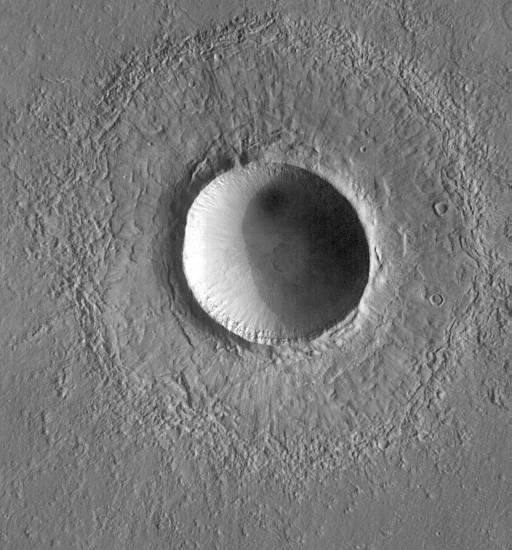
\includegraphics[width=\textwidth,keepaspectratio]{images/Gre13/Gre13_01.jpg}
		\captionsetup{format=plain,width=0.85\textwidth}
		\caption{Eingabebild, aus \cite[Kap.~7]{greeley_13}}
		\label{fig:slic_vs_tsugf_in}
	\end{subfigure}
	\hfill
	\begin{subfigure}[t]{0.32\textwidth}
		\centering
		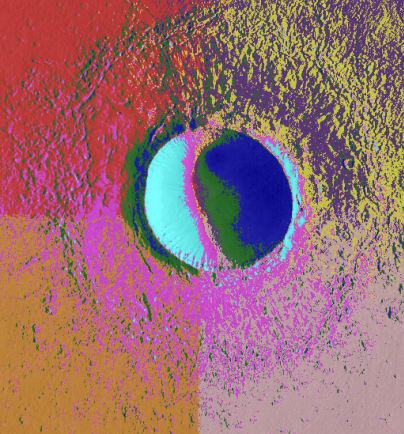
\includegraphics[width=\textwidth,keepaspectratio]{images/gen/slic_vs_tsugf/Gre13_01.jpg_slic.png}
		\captionsetup{format=plain,width=0.85\textwidth}
		\caption{Ergebnis des SLIC-Algorithmus \cite{achanta_10} angewandt auf die Eingabedatei}
		\label{fig:slic_vs_tsugf_slic}
	\end{subfigure}
	\hfill
	\begin{subfigure}[t]{0.32\textwidth}
		\centering
		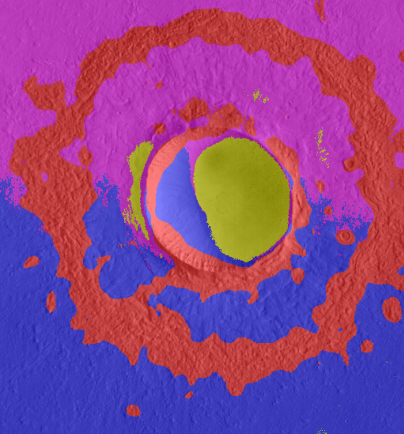
\includegraphics[width=\textwidth,keepaspectratio]{images/gen/slic_vs_tsugf/Gre13_01.jpg_tsugf.png}
		\captionsetup{format=plain,width=0.85\textwidth}
		\caption{Ergebnis des texturbasierten Clusterings (\vgl Unterabschnitt~\ref{ssec:tsugf}) der Eingabedatei}
		\label{fig:slic_vs_tsugf_tsugf}
	\end{subfigure}
	\caption{Clustering eines Graustufenbildes eines Kraters der Marsoberfläche}
\end{figure}

So ergibt ein Clustering des Kraters aus Unterabschnitt~\ref{ssec:mars_surface_features} durch den SLIC-Algorithmus \cite{achanta_10} das in \figurename~\ref{fig:slic_vs_tsugf_slic} sichtbare Ergebnis.\footnote{SLIC-Implementierung: \texttt{scikit-image}\\Parameter: \texttt{compactness=5, n\_segments=10, enforce\_connectivity=False}} Dort ist erkennbar, dass der Krater in jeweilige Licht- und Schattenregionen (bedingt durch den Lichteinfall im flachen Winkel) unterteilt wird. Außerdem wird die raue Struktur ringförmig um den Krater herum schlecht erfasst: An dieser Stelle wird jeder Hügel separat als einerseits helle, andererseits dunkle Stelle markiert. Das Phänomen, dass ein Krater durch eine starke Differenz an Licht- und Schattenregionen erkannt wird wird sich im Großen und Ganzen zwar in Abschnitt~\ref{sec:crater_detection} zu nutze gemacht, ist hier allerdings ungewollt.

Wenn nun der in Unterabschnitt~\ref{ssec:kanezaki} beschriebene Ansatz verfolgt wird, wird das neuronale Netz daraufhin trainiert, eine Aufnahme anhand ihrer Helligkeitsinformationen hin zu trainieren. Da dies nicht gewollt ist, wird statt einem farb-/helligkeitsbasierten Clusteringalgorithmus wie SLIC ein texturbasiertes Clustering genutzt.

Statt des SLIC-Clusterings wird nun die in Unterabschnitt~\ref{ssec:tsugf} vorgestellte Methode des texturbasierten Clusterings genutzt. Von dieser Stelle an sind, wenn nicht anders benannt, die Gewichtungen der verschiedenen Werte für die Farbwerte, X-/Y-Positionen und Reaktion auf Gaborfilter alle gleich $1$. Diese Parameter werden in Unterabschnitt~\ref{ssec:initialization_filterweight} genauer erläutert.

Das Resultat eines Clusterings durch die genutzte, texturbasierte Methode\footnote{Kombiniert mit der Filterbank aus \cite{jain_91}} ist in \figurename~\ref{fig:slic_vs_tsugf_tsugf} sichtbar: Man erkennt, dass der \enquote{Ring} um den eigentlichen Einschlagskrater eine eigenständige Textur besitzt, welche unterschiedlich zu dem Rest der Oberfläche ist. Eine ähnliche Oberflächenstruktur ist direkt um den Krater herum vorhanden. Beide Vorkommnisse dieser ähnlichen Struktur werden vom texturbasierten Clustering erfasst, in ein Segment aufgeteilt und (hier durch eine rote Färbung) markiert.

% TODO Reread

\subsection{Filterbänke}
\label{ssec:initialization_filterbanks}
An dieser Stelle stellt sich die Frage, welche der vorgestellten Filterbänke sich gut eignet, die Eingabedatei zu clustern. Die größten Unterschiede zwischen den einzelnen Filterbänken besteht darin, dass einige von ihnen rotationsinvariante Filter enthalten, und andere in mehreren Größen vorhanden sind. Die Größendifferenz lässt sich in der Anwendung des Algorithmus dadurch ausgleichen, dass jeder Filter zusätzlich in weitere Größen skaliert wird, und in jeder Skalierungsstufe angewandt wird. Die Rotationsinvarianz würde sich höchstens durch die Rotation der Filter approximieren lassen, da so allerdings nicht jeder Winkel abgedeckt werden kann, ist diese Methode ungeeignet. Ein Vergleich verschiedener Filterbänke ist in Unterabschnitt~\ref{ssec:exp_filterbanks} zu finden.

\subsection{Größe der Filter}
\label{ssec:initialization_filtersize}

Neben der Auswahl einer geeigneten Filterbank lassen sich in dieser noch die einzelnen Gewichtungen anpassen: So könnten \zB die Gewichtung der Koordinaten der Pixel zueinander oder die Relevanz von ähnlichen Farbwerten modifiziert werden. Außerdem ist die Größe der einzelnen Filter in den jeweiligen Filterbänken auch Variabel und muss dementsprechend an die Dimensionen des jeweiligen Eingabebildes angepasst werden. Da alle Filterbänke (bis auf die nach \cite{jain_91}) jeweils gleiche Filter in unterschiedlichen Größen enthalten, muss nur ein Gesamtwert angepasst werden, statt der Größe jeder einzelnen Skalierung. 

Der Skalierungsfaktor $s$ gibt an, mit welchem Faktor die ursprüngliche Seitenlänge des Filters multipliziert wird, $s=1$ bedeutet somit, dass der Filter eine Seitenlänge von \SI{49}{\pixel} beibehält. In Unterabschnitt~\ref{ssec:exp_filtersize} werden unterschiedliche Skalierungsfaktoren verglichen.

\subsection{Gewichtungen der Parameter}
\label{ssec:initialization_filterweight}

Da in dem Prozess des Clusterings alle Optimierungen aus Unterabschnitt~\ref{ssec:tsugf} miteingeschlossen sind, verarbeitet k-Means einen Datenwürfel, welcher auch die Koordinaten und Farbwerte der jeweiligen Pixel miteinbeschließt. Nun stellt sich die Frage, wie stark diese jeweils gewichtet werden sollten, um ein akzeptables Ergebnis zu erhalten. Aus diesem Grund sind in Unterabschnitt~\ref{ssec:exp_filterweight} ie Resultate des Clusterings mit unterschiedlichen Werten für die jeweiligen Gewichtungen zu sehen.

\subsection{Anzahl der Cluster}
\label{ssec:initialization_number_of_segments}

Bis zu dieser Stelle haben sich vier Cluster sehr gut zur Visualisierung der unterschiedlichen Ergebnisse nutzen lassen, dies ändert sich allerdings wenn die jeweiligen Clusterings an das darauf folgende neuronale Netz weitergegeben werden. Die Anzahl der Cluster mit denen begonnen werden soll ist ein entscheidender Wert bei dem Prozess der Segmentierung: Ist diese Zahl zu gering, kann das Netzwerk dieses Clustering nicht weiter verfeinern, ist sie jedoch zu groß, so sind innerhalb eines Clusters nicht genug Informationen vorhanden, als dass das Netzwerk erlernen kann, nach welchen Kriterien das Bild ursprünglich aufgeteilt wurde. Ein Vergleich unterschiedlicher Werte für diese Anzahl der Startcluster ist in Unterabschnitt~\ref{ssec:exp_number_of_segments} sichtbar.

\section{Algorithmus}
\label{sec:algorithm}

Der Algorithmus aus \cite{kanezaki_18}, also das Füllen der Cluster der dynamisch erstellen Zielsegmentierung mit den derzeitigen Werten, wird größtenteils unverändert gelassen. Eine Modifikation die sich allerdings doch als hilfreich erwiesen hat, ist dass dieser genannte Vorgang nicht in jeder Iteration des Netzes geschieht, sondern nur alle $n$ Iterationen. Dies ermöglicht dem Netzwerk mehr Epochen zum Lernen der Methodik jeweiligen Segmentierung, bevor diese wieder verändert wird.

\section{Netzwerkarchitektur}
\label{sec:network_architecture}

Die Netzwerkarchitektur im originalen Paper stellt ein einfaches Netzwerk zur Objekterkennung oder Bildsegmentierung dar: Es durchläuft iterativ drei mal eine Reihe mit je einer Convolutional Layer, gefolgt von einer Batch Normalization. Im Folgenden wird geprüft, ob eine Modifikation dieser Architektur in diesem domänenspezifischen Anwendungsfall zu Verbesserungen der Ergebnisse führen kann. Für die Initialisierung werden die im letzten Kapitel erläuterten Parameter genutzt.

\subsection{Abbruchkriterium}
\label{ssec:stoppingcriteria}

Die originale Implementierung nutzt die Anzahl der Segmente, die das neuronale Netz erzeugt, als Abbruchkriterium für das Netzwerk. Ist diese geringer als ein im Vorhinein festgelegter Wert, so wird das Training des Netzes gestoppt und die aktuelle Segmentierung als Ergebnis ausgegeben. Neben dieser simplen Methode lässt sich auch der Wert der Verlustfunktion als Abbruchkriterium nutzen. Da dieser allerdings pro Eingabedatei unterschiedlich zueinander ausfällt, kann dieser nicht direkt genutzt werden.

Eine Lösungsmöglichkeit besteht daraus, den Median der relativen Änderung zur jeweils vorherigen Epoche in den letzten $n$ Epochen zu betrachten. Diese Änderungsrate sinkt während der Laufzeit des Training, da die weitere Optimierung der Segmentierung immer geringer ausfällt. Die Wahl von $n$ ist entscheidend für die erfolgreiche Funktionsweise dieser Methode, da ein zu kleiner Wert bedeuten könnte, dass das Netzwerk abgebrochen wird, wenn vorzeitig eine lokale Extremstelle auftritt, also \zB innerhalb von einigen Epochen wenig neue Informationen gelernt werden. Ist $n$ allerdings zu groß, werden zu viele Epochen betrachtet, sodass eine aktuelle Senkung dieser Änderung erst spät bemerkt wird.

Ein weiterer Ansatz zur Lösung dieses Problems ist die Nutzung des Wertes der Ableitung der Verlustfunktion in der aktuellen Epoche. Dies ist allerdings nicht direkt möglich, da die Verlustfunktion nicht stetig definiert ist, sondern nur an den Stellen der jeweiligen Epochen. Dies lässt sich dadurch ausgleichen, dass die bekannten Punkte durch eine stetige Funktion approximiert werden, welche anschließend abgeleitet werden kann.

Der Vergleich dieser Abbruchkriterien ist in Unterabschnitt~\ref{ssec:exp_stoppingcriteria} aufgeführt.

\subsection{Aktivierungsfunktionen}
\label{ssec:network_architecture_activation}

In der originalen Implementierung nach \cite{kanezaki_18} enthält das neuronale Netz die ReLU-Funktion als Aktivierungsfunktion vor der Batch Normalization-Layer.Es wird nun untersucht, ob das Entfernen oder Ersetzen einer solchen Aktivierungsfunktionen die Clusteringergebnisse verbessern kann.

In Unterabschnitt~\ref{ssec:exp_architecture_activation} werden die am weitesten verbreiteten Aktivierungsfunktionen verglichen: Die ReLU-, die Sigmoid- und die tanh-Funktion (\vgl Unterabschnitt~\ref{ssec:activation_layer}). Außerdem wird geprüft, ob das Entfernen der vorhandenen ReLU-Funktion zu einer Verbesserung der Ergebnisse führen kann.

\subsection{Pooling Layer}
\label{ssec:network_architecture_pooling}

Auch auf Pooling Layers wurde im ursprünglichen Paper verzichtet. Pooling Layers können, wie in Unterabschnitt~\ref{ssec:pooling_layer} beschrieben, dabei helfen, Informationen aus verschiedenen Bildbereichen zu abstrahieren und aggregieren, es könnte also in dieser Hinsicht zu besseren Ergebnissen führen. Ein Problem allerdings ist, dass Pooling Layers die Auflösung des Bildes merklich verringern, wird solch eine Schicht \bspw mit einer Kernelgröße von $F_1=F_2=2$ genutzt, enthält die Ausgabe nur ein Viertel der Pixel der Eingabedatei. Dies ist zwar ein geringeres Problem bei der Objekterkennung, kann allerdings bei der Segmentierung, bei welcher es auf die möglichst genaue Bestimmung der Kanten von Strukturen ankommt, zu einer Genauigkeitseinbüßung führen. Außerdem kann je nach Kernelgröße und weiteren Hyperparametern der Fall eintreten, dass sehr feine Oberflächenmerkmale durch das Pooling verloren gehen. Die Entsprechenden Resultate dieser Experimente sind in Unterabschnitt~\ref{ssec:exp_architecture_pooling} zu finden.

\subsection{Fully Connected Layers}
\label{ssec:network_architecture_fully_connected}

Wie in Unterabschnitt~\ref{ssec:fully_connected_layer} werden Fully Connected Layers in Convolutional Neural Networks dazu eingesetzt, die Resultate der ihr vorhergehenden Schichten zu klassifizieren. Angewandt auf das hier genutzte Netzwerk könnte ihre Nutzung zur Folge haben, dass verschiedene lokale Oberflächenmerkmale besser im globalen Kontext erkannt werden können und \ggf in die selben Cluster wie ihnen ähnliche Regionen eingeteilt werden. Ob dies auch in der praktischen Anwendung der Fall ist, wird in Unterabschnitt~\ref{ssec:exp_fully_connected} erläutert.


\iffalse

\section{Hyperparameter}
\label{sec:hyperparameter}


\subsection{Merkmalsdimensionen}

Die Anzahl der Merkmalsdimensionen $n_{fd}$ gibt (hier) die Anzahl der Schichten an, welcher der Datenwürfel, welcher bei der Konvolution generiert wird, besitzt. Anders ausgedrückt, ist er gleich der Anzahl der genutzten Kernel einer Konvolutions-Schicht. In der Beispielimplementierung nach \cite{kanezaki_18} wird von ein Standardwert von $n_{fd} = 100$ ausgegangen. Im Folgenden wird anhand der \figurename~\ref{fig:fd_comparision} überprüft, ob sich dieser Wert für den hier genutzten Anwendungsfall optimieren lässt.

\begin{figure}[h!]
	\setlength\tabcolsep{1pt}
	\def\arraystretch{0.5}
	\begin{tabular}{m{15pt}m{0.166\textwidth}m{0.166\textwidth}m{0.166\textwidth}m{0.166\textwidth}m{0.166\textwidth}m{0.166\textwidth}}
		\texttt{a)} &
		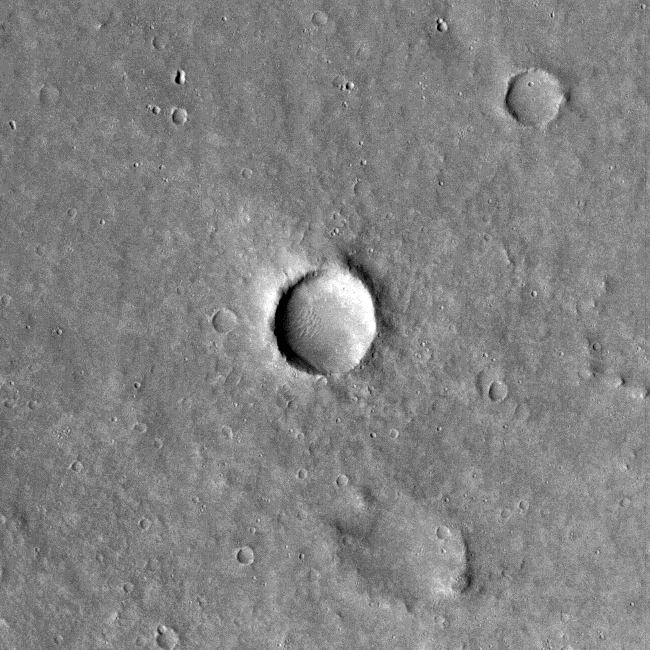
\includegraphics[width=0.15\textwidth]{images/p03/p03_01.png} &
		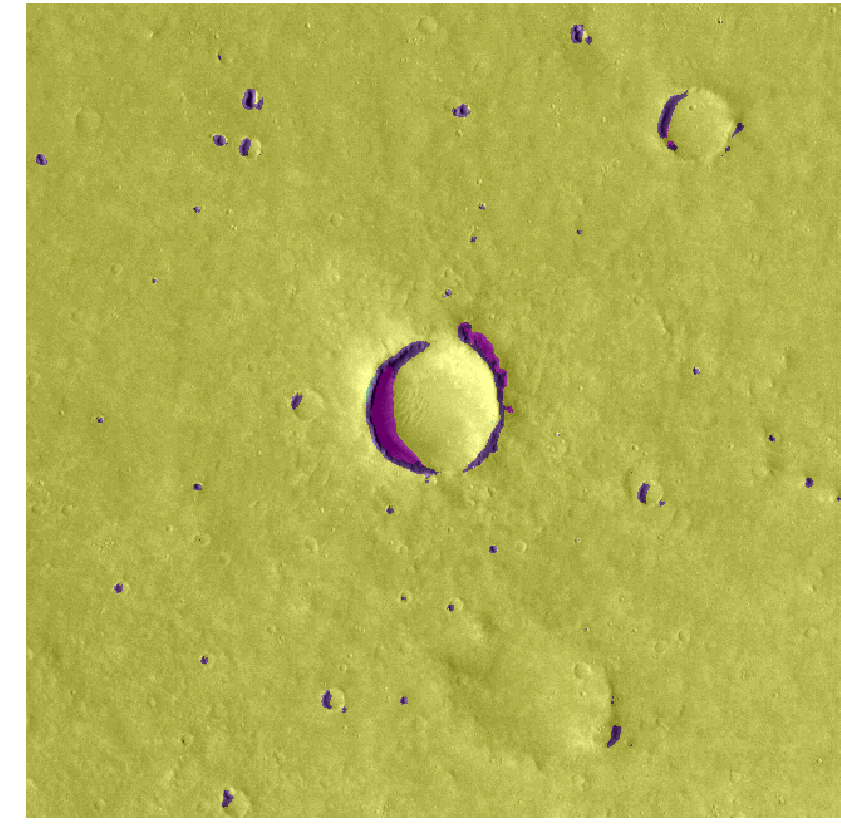
\includegraphics[width=0.15\textwidth]{images/gen/feature_dimensions/p03_01.png_33.png} &
		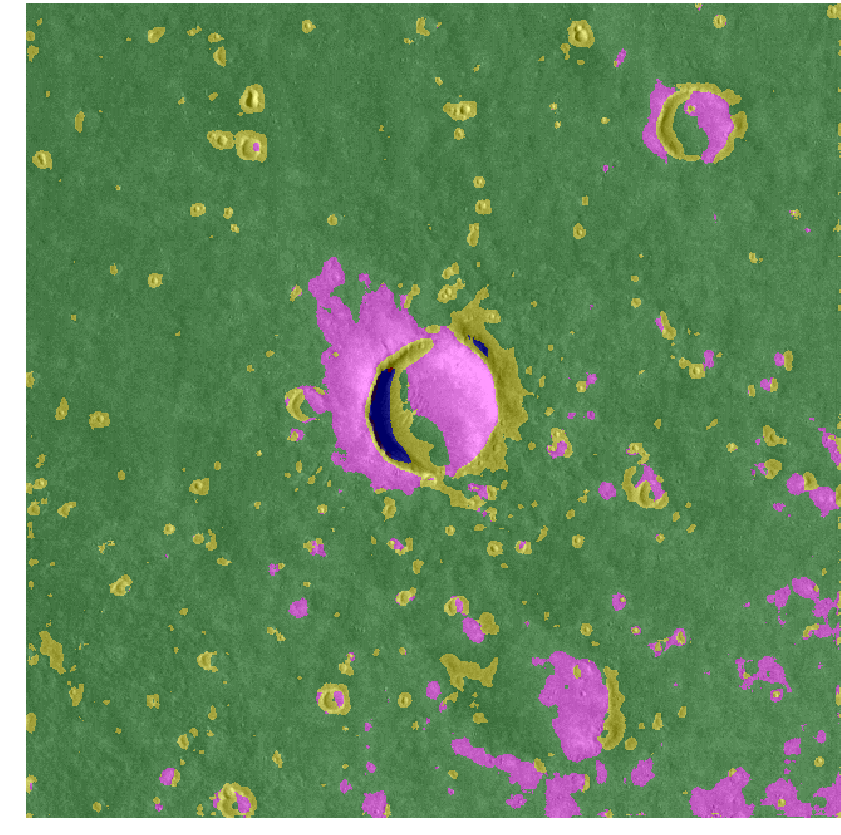
\includegraphics[width=0.15\textwidth]{images/gen/feature_dimensions/p03_01.png_67.png} &
		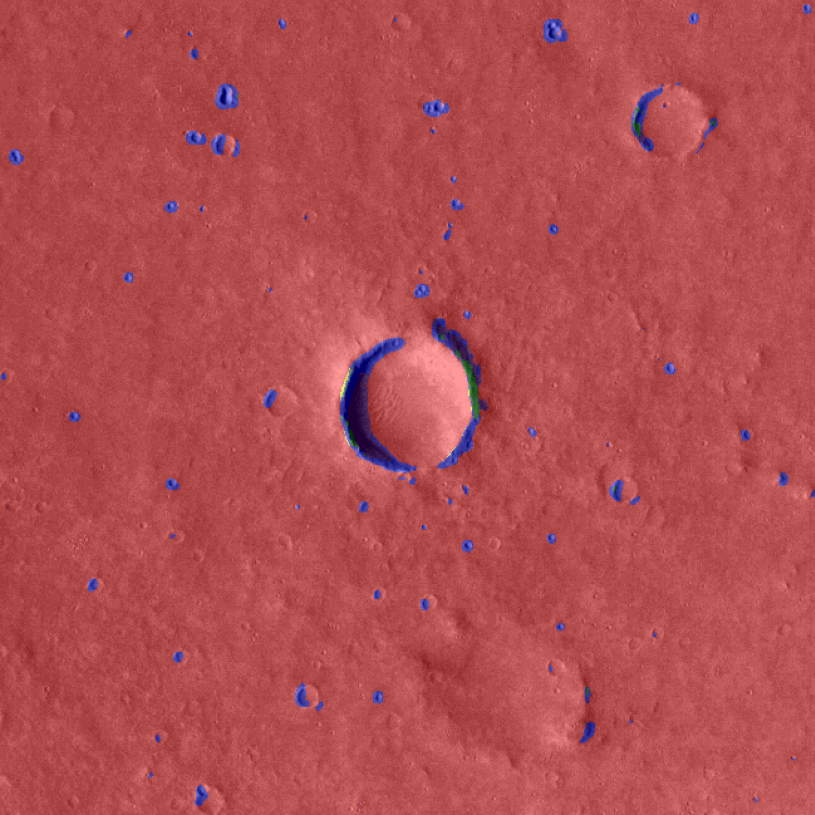
\includegraphics[width=0.15\textwidth]{images/gen/feature_dimensions/p03_01.png_100.png} &
		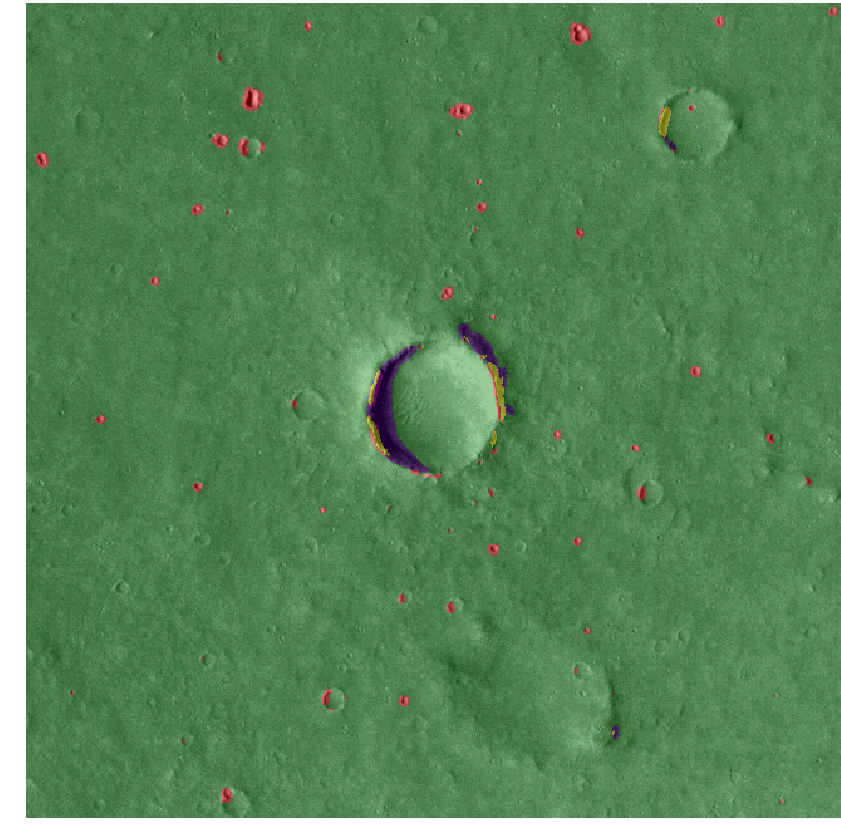
\includegraphics[width=0.15\textwidth]{images/gen/feature_dimensions/p03_01.png_133.png} &
		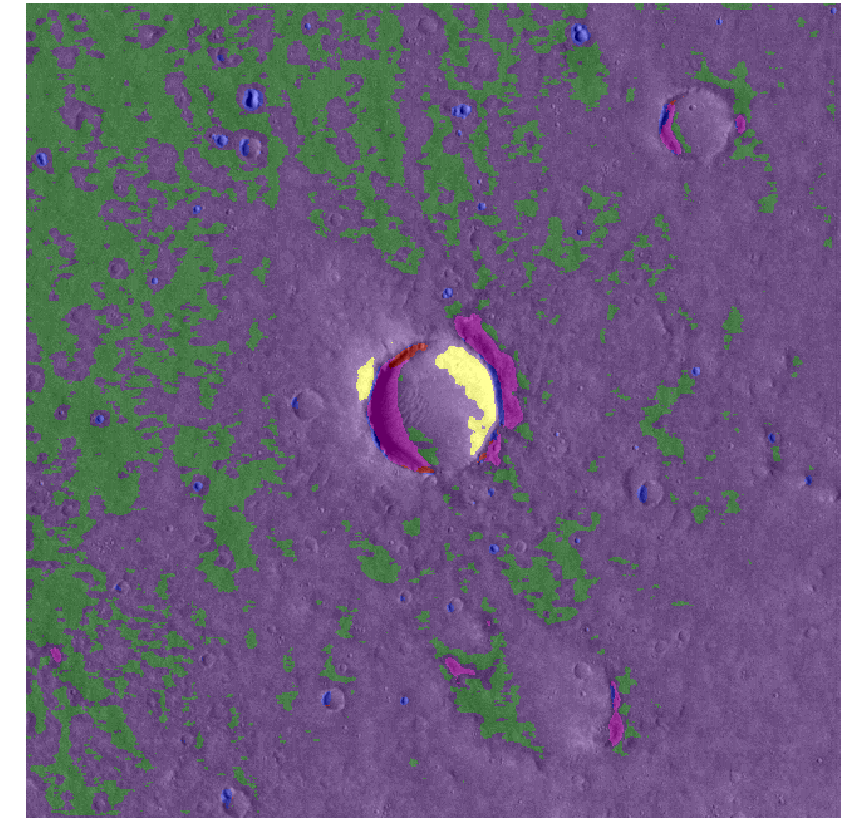
\includegraphics[width=0.15\textwidth]{images/gen/feature_dimensions/p03_01.png_167.png} \\
		\texttt{b)} &
		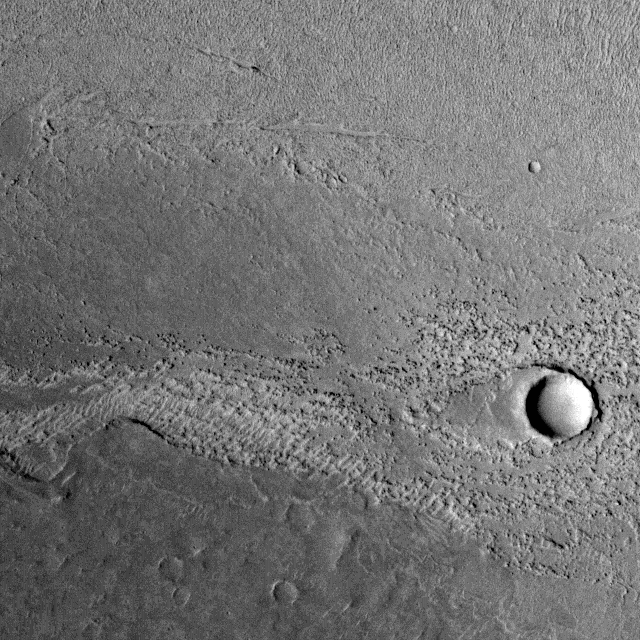
\includegraphics[width=0.15\textwidth]{images/p03/p03_02.png} &
		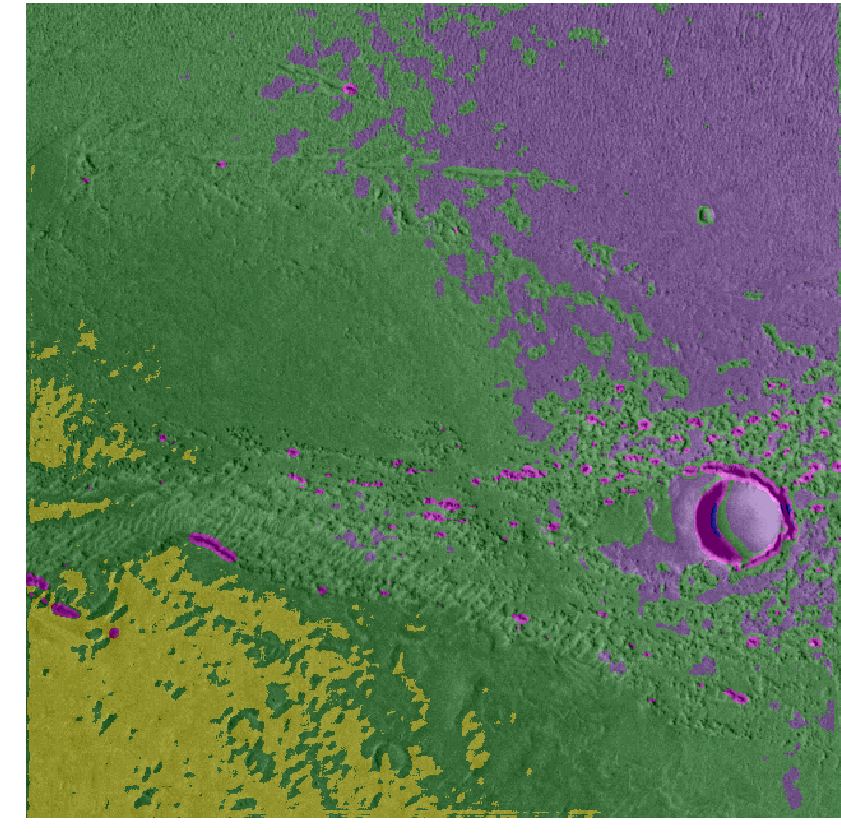
\includegraphics[width=0.15\textwidth]{images/gen/feature_dimensions/p03_02.png_33.png} &
		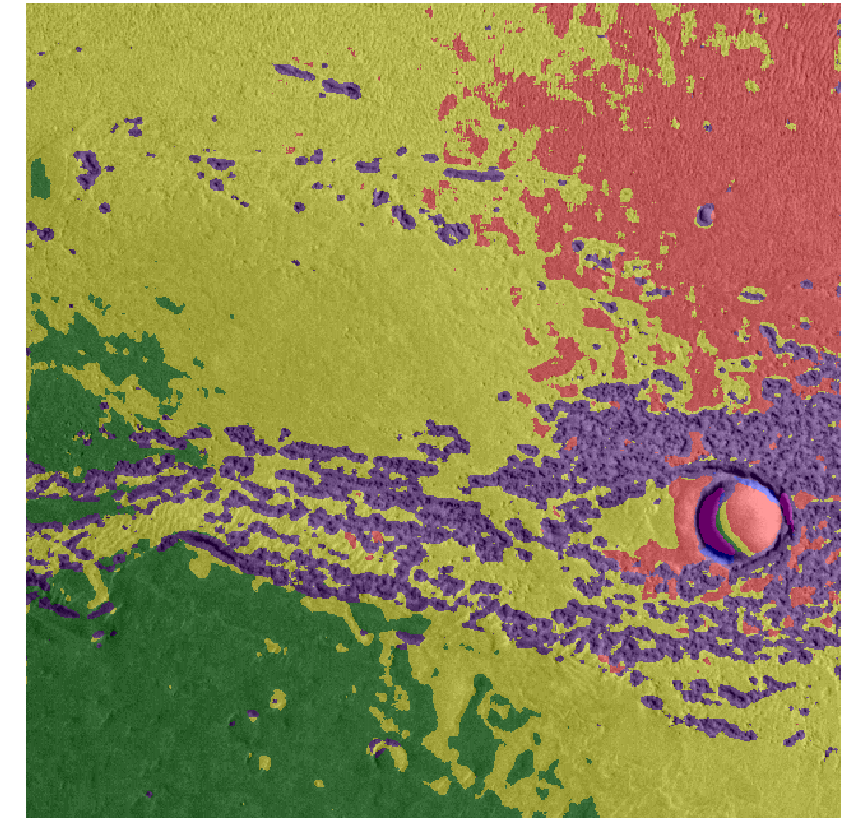
\includegraphics[width=0.15\textwidth]{images/gen/feature_dimensions/p03_02.png_67.png} &
		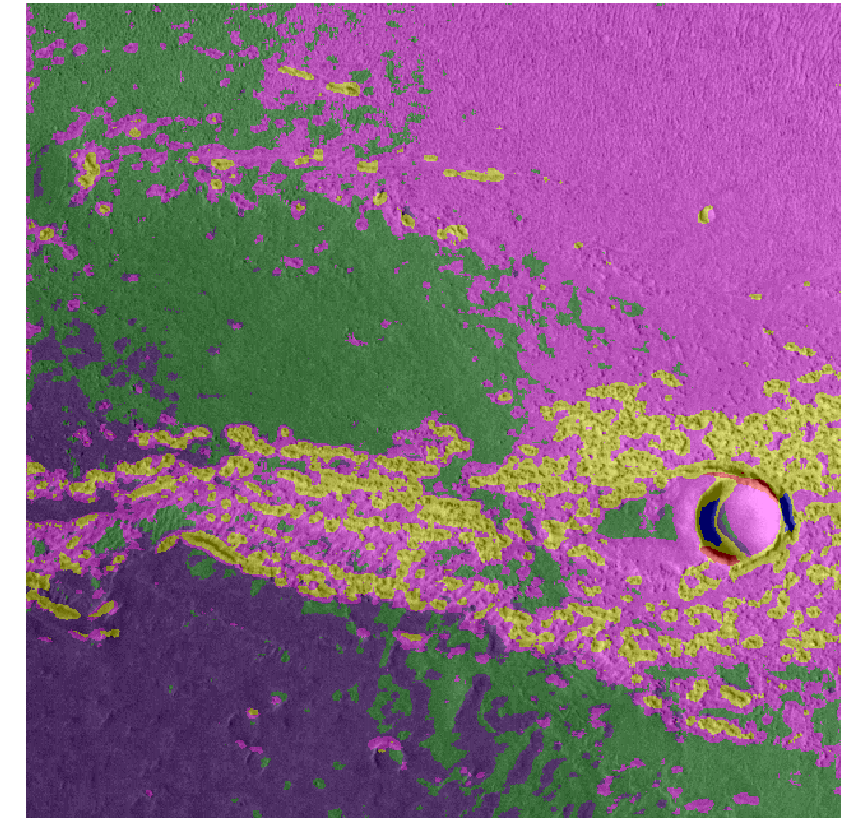
\includegraphics[width=0.15\textwidth]{images/gen/feature_dimensions/p03_02.png_100.png} &
		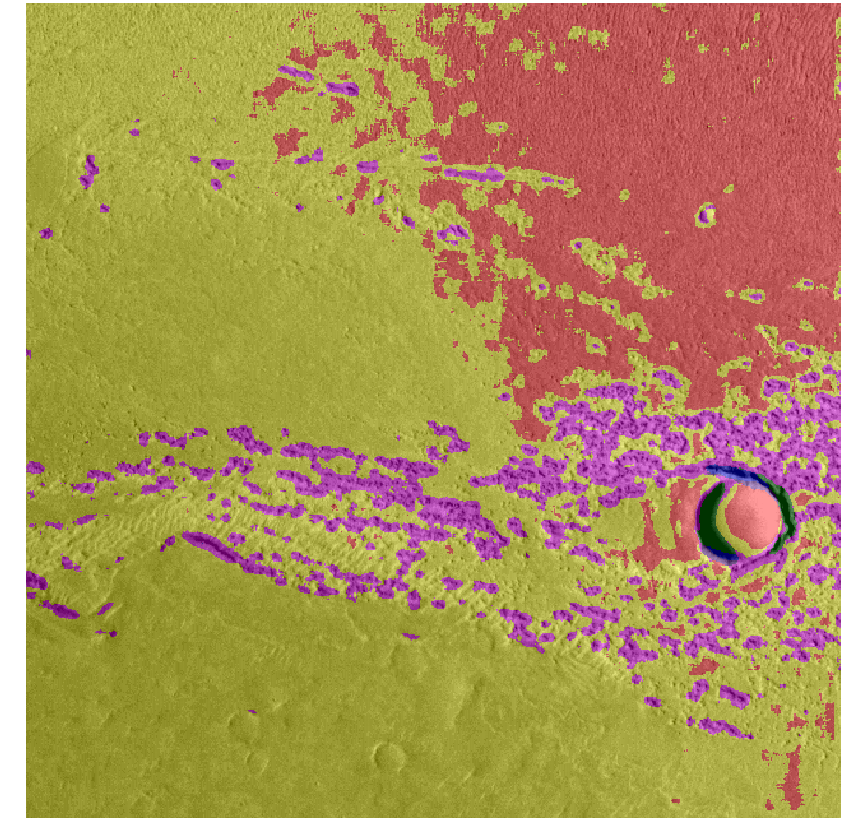
\includegraphics[width=0.15\textwidth]{images/gen/feature_dimensions/p03_02.png_133.png} &
		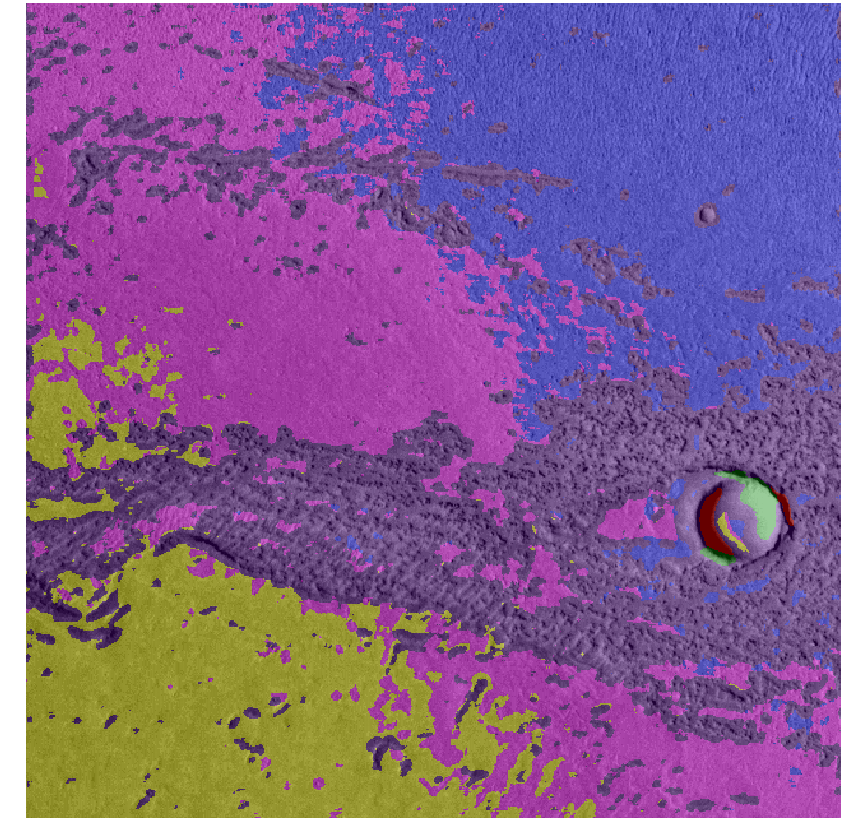
\includegraphics[width=0.15\textwidth]{images/gen/feature_dimensions/p03_02.png_167.png} \\
		\texttt{c)} &
		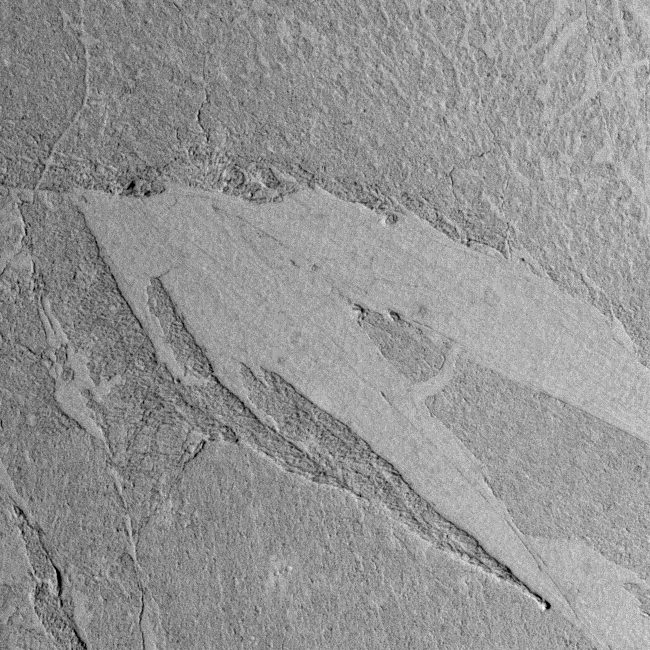
\includegraphics[width=0.15\textwidth]{images/p03/p03_03.png} &
		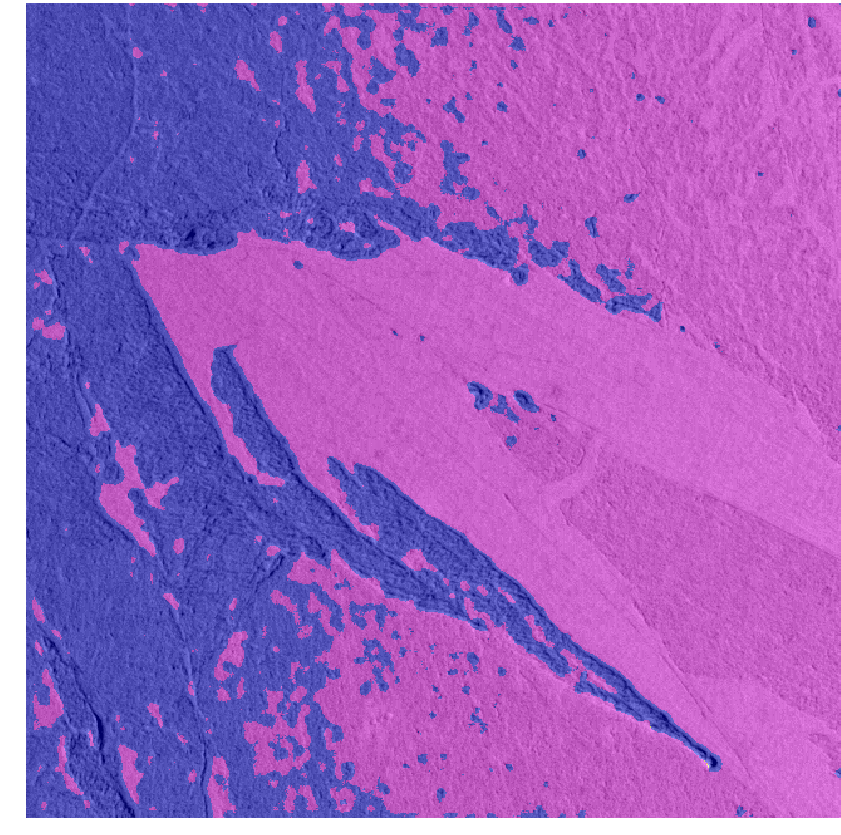
\includegraphics[width=0.15\textwidth]{images/gen/feature_dimensions/p03_03.png_33.png} &
		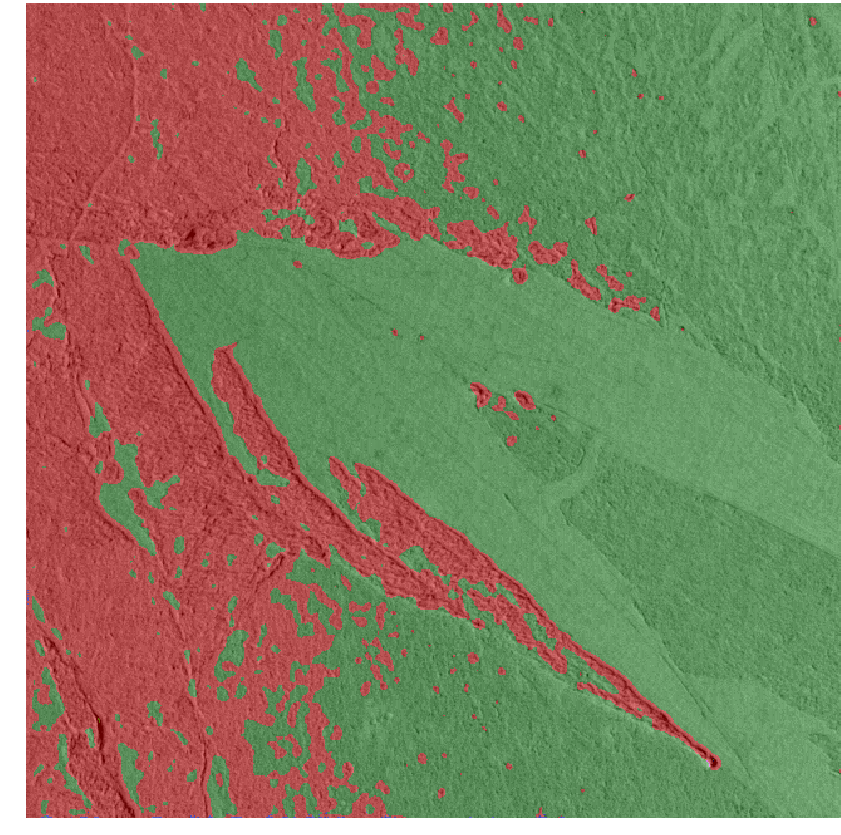
\includegraphics[width=0.15\textwidth]{images/gen/feature_dimensions/p03_03.png_67.png} &
		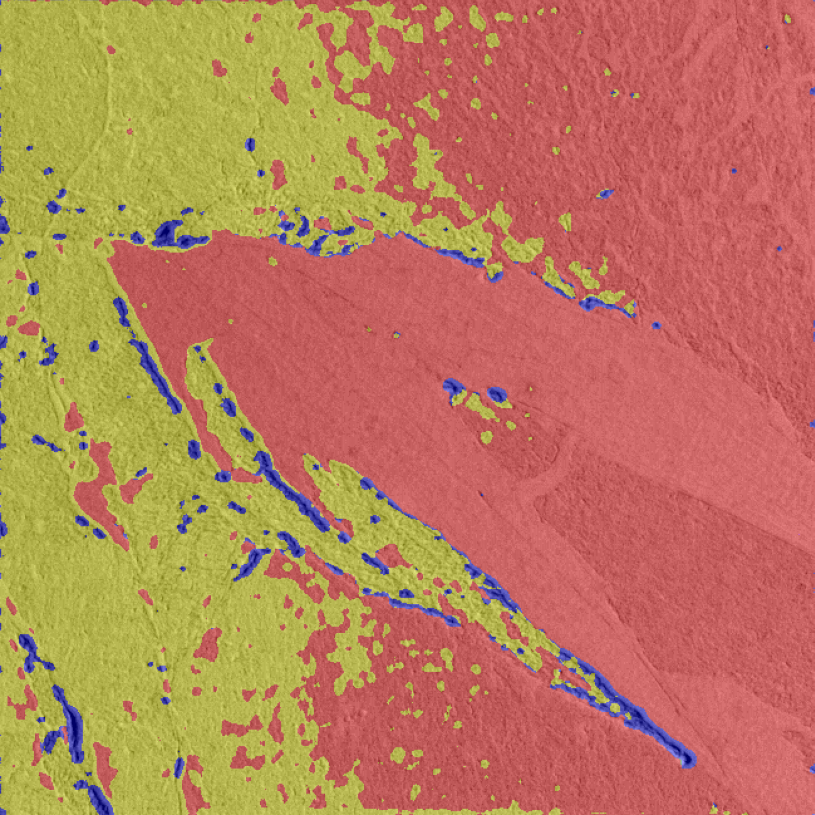
\includegraphics[width=0.15\textwidth]{images/gen/feature_dimensions/p03_03.png_100.png} &
		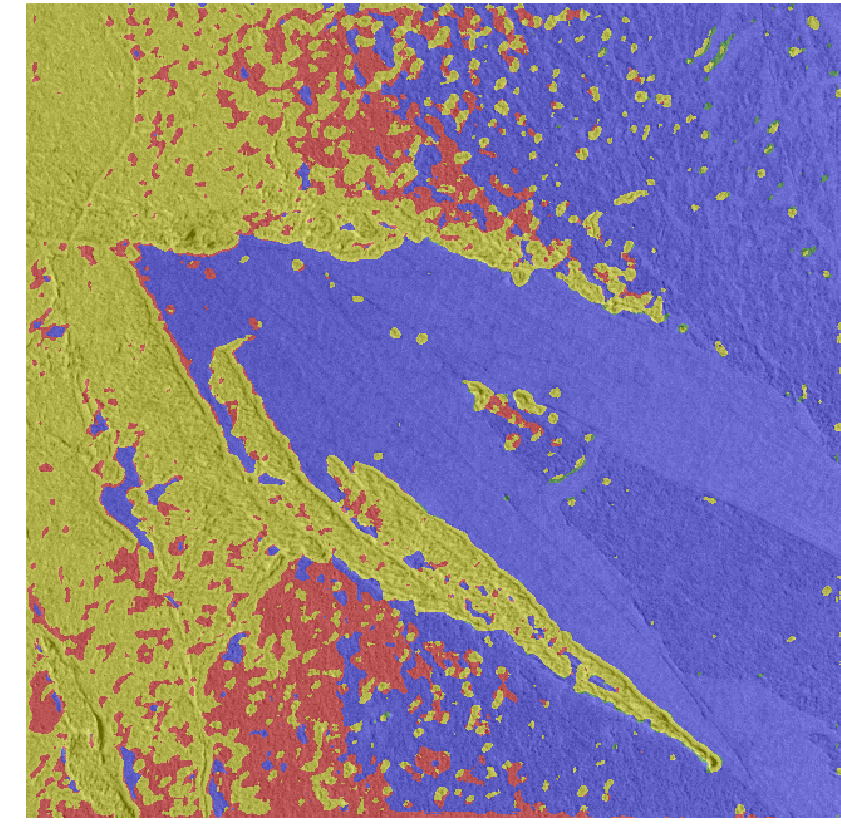
\includegraphics[width=0.15\textwidth]{images/gen/feature_dimensions/p03_03.png_133.png} &
		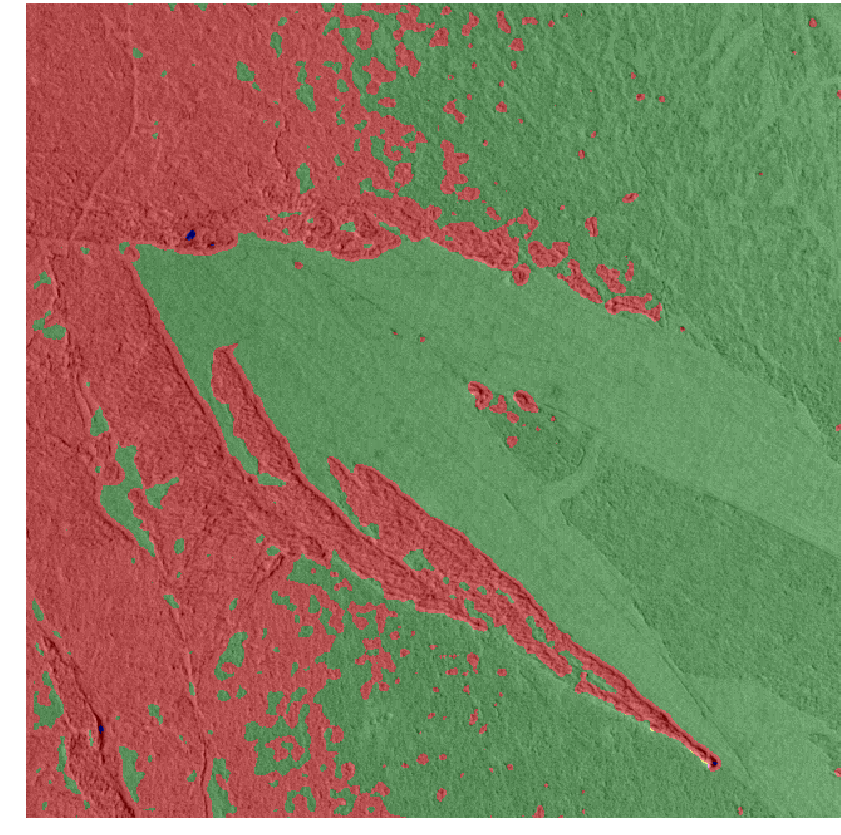
\includegraphics[width=0.15\textwidth]{images/gen/feature_dimensions/p03_03.png_167.png} \\
		\texttt{d)} &
		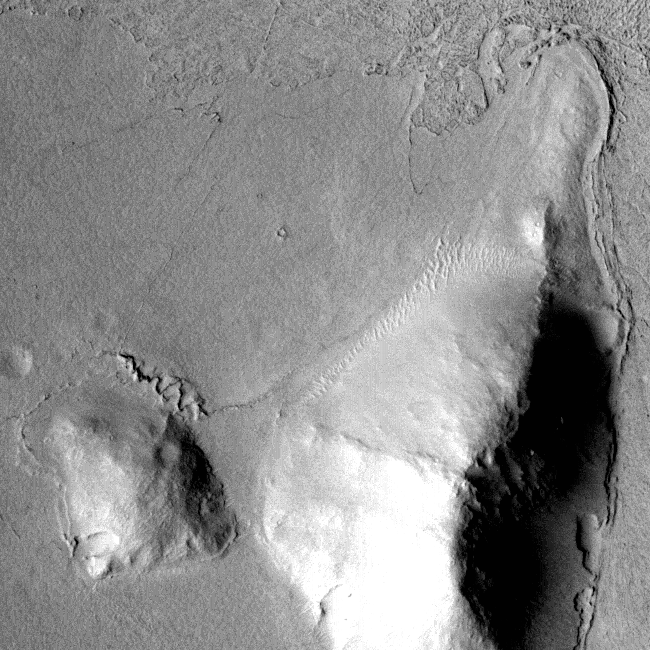
\includegraphics[width=0.15\textwidth]{images/p03/p03_04.png} &
		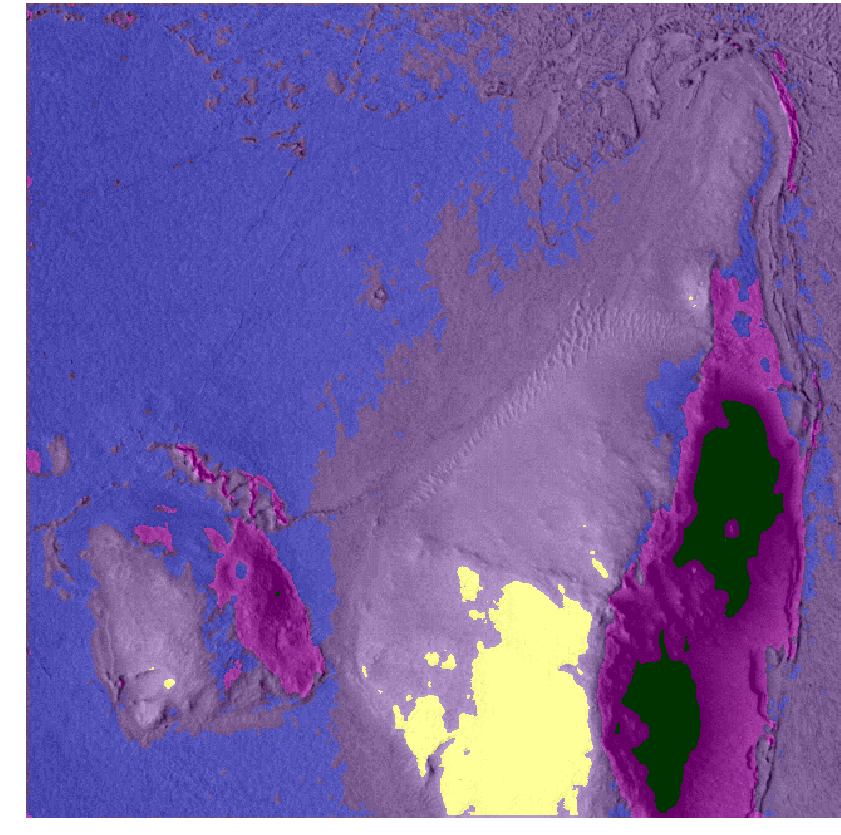
\includegraphics[width=0.15\textwidth]{images/gen/feature_dimensions/p03_04.png_33.png} &
		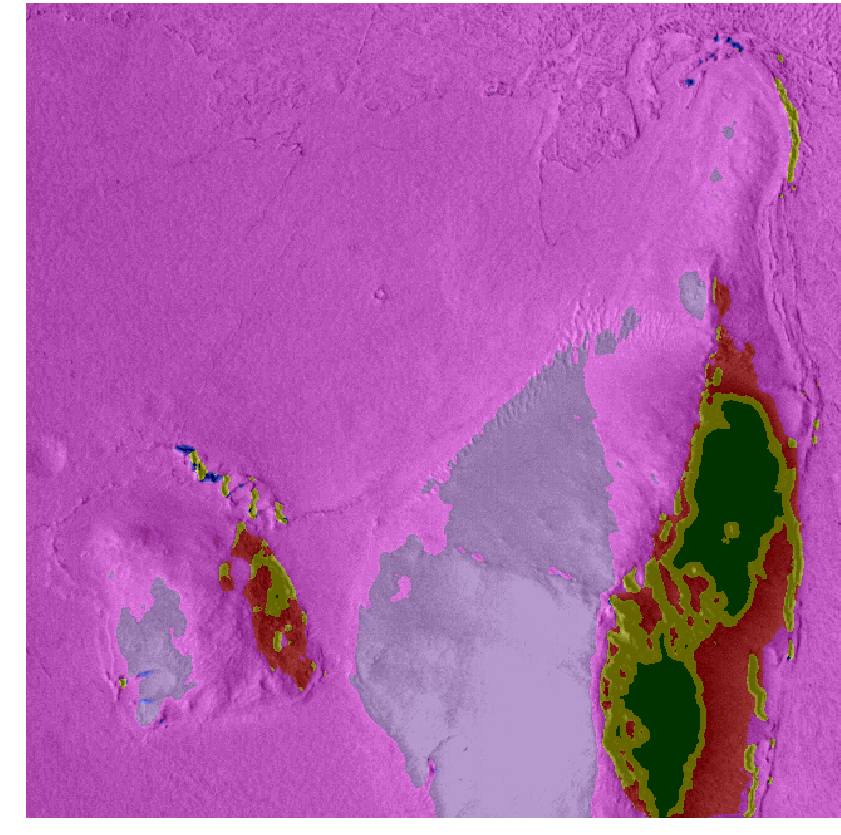
\includegraphics[width=0.15\textwidth]{images/gen/feature_dimensions/p03_04.png_67.png} &
		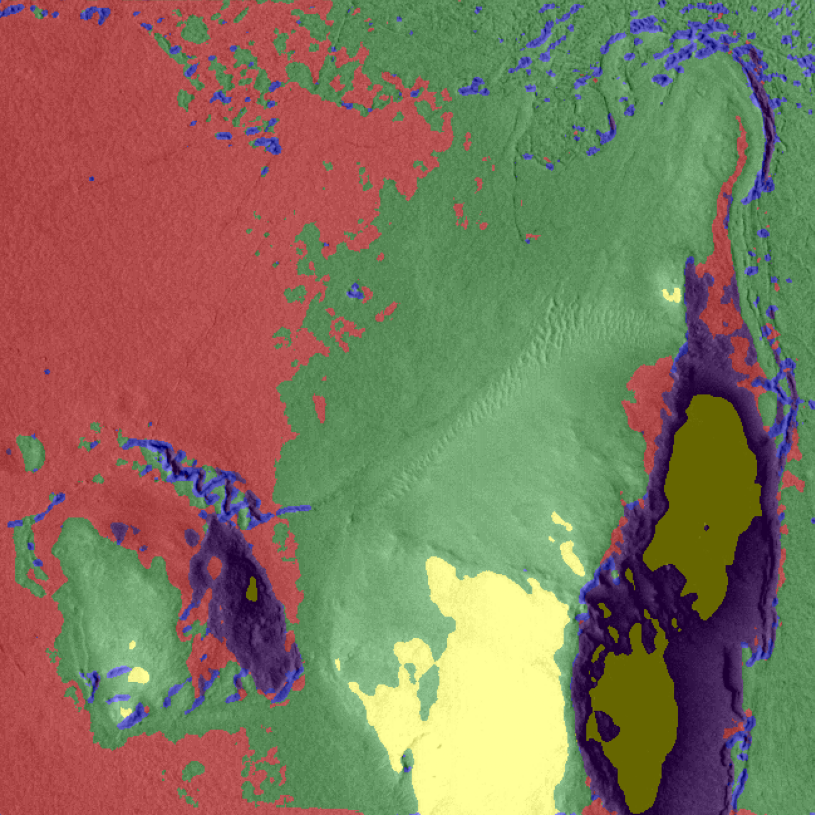
\includegraphics[width=0.15\textwidth]{images/gen/feature_dimensions/p03_04.png_100.png} &
		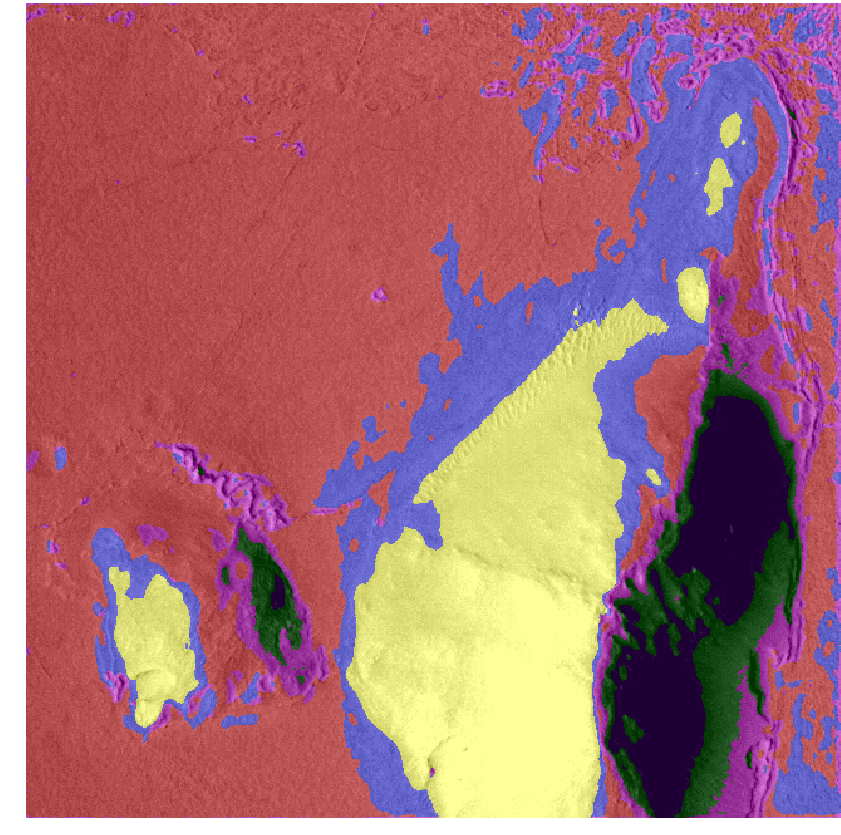
\includegraphics[width=0.15\textwidth]{images/gen/feature_dimensions/p03_04.png_133.png} &
		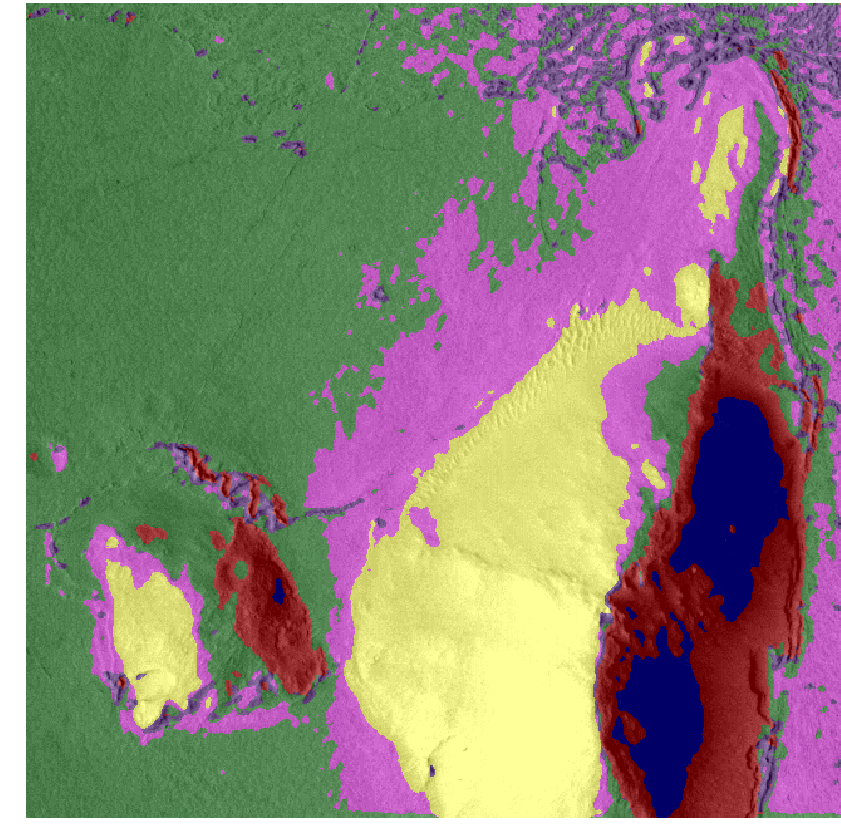
\includegraphics[width=0.15\textwidth]{images/gen/feature_dimensions/p03_04.png_167.png} \\
		
		&
		\vspace*{2pt}\centering Eingabe & 
		\vspace*{2pt}\centering $n_{fd}=33$ &
		\vspace*{2pt}\centering $n_{fd}=67$ &
		\vspace*{2pt}\centering $n_{fd}=100$ &
		\vspace*{2pt}\centering $n_{fd}=133$ &
		\vspace*{2pt}\centering $n_{fd}=167$ \\
	\end{tabular}
	\caption{Vergleich der Auswirkungen einer veränderten Anzahl an Merkmalsdimensionen. Die Farben der jeweiligen Cluster wurden zufällig gewählt.}
	\label{fig:fd_comparision}
\end{figure}
\fi
\subsection{Anzahl der Konvolutionsschichten}

In der originalen Implementierung war die Anzahl der Konvolutionsschichten (gefolgt von den Aktivierungs- und Batch-Normalisierungs-Schichten) dynamisch, mit einem Standardwert von drei Schichten. Nun wird über \figurename~\ref{fig:n_layers_comparision} überprüft, welchen Einfluss eine Veränderung dieses Parameters auf die entstehende Segmentierung hat.

\begin{figure}[h!]
	\setlength\tabcolsep{1pt}
	\def\arraystretch{0.5}
	\begin{tabular}{m{15pt}m{0.166\textwidth}m{0.166\textwidth}m{0.166\textwidth}m{0.166\textwidth}m{0.166\textwidth}m{0.166\textwidth}}
		\texttt{a)} &
		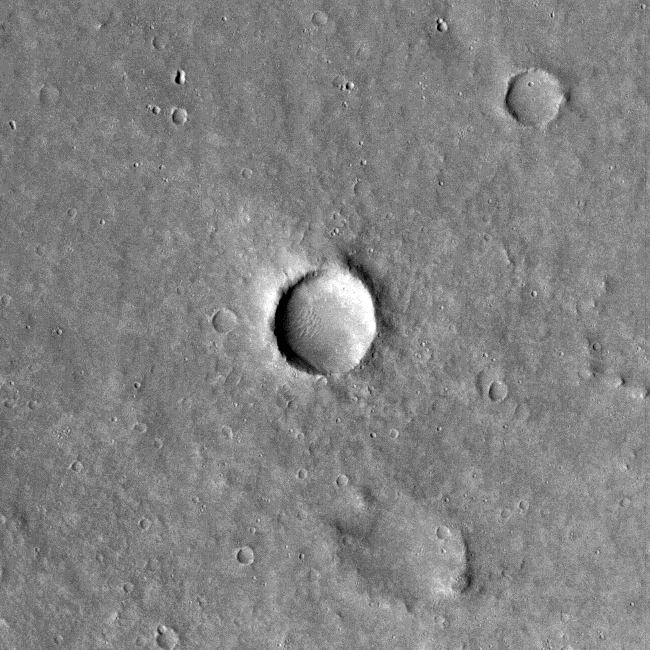
\includegraphics[width=0.15\textwidth]{images/p03/p03_01.png} &
		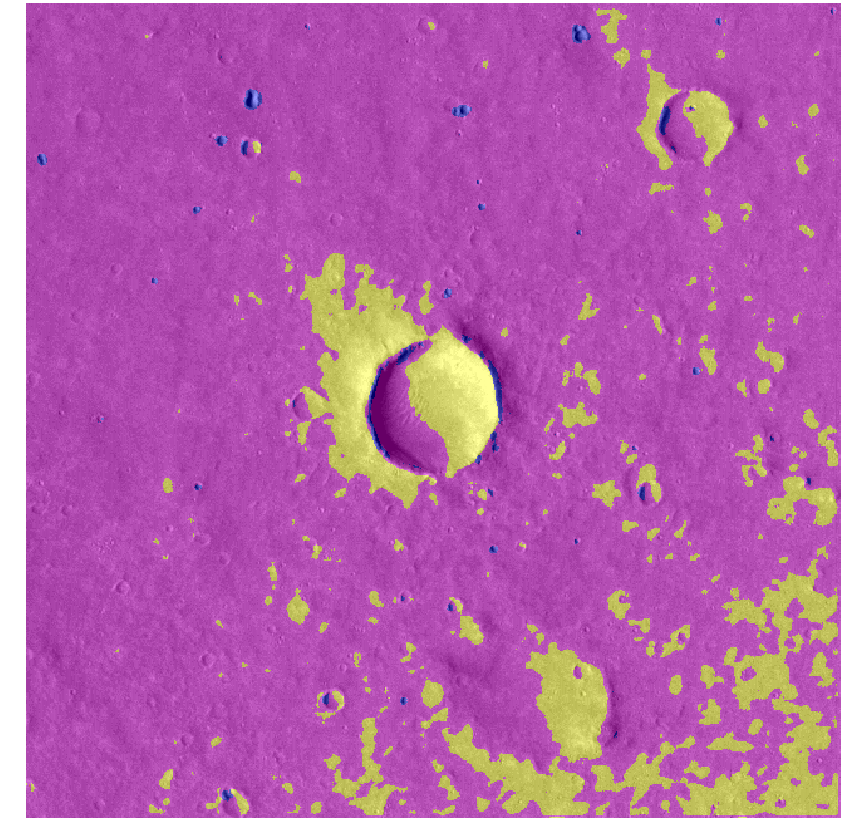
\includegraphics[width=0.15\textwidth]{images/gen/convolution_number/p03_01.png_2.png} &
		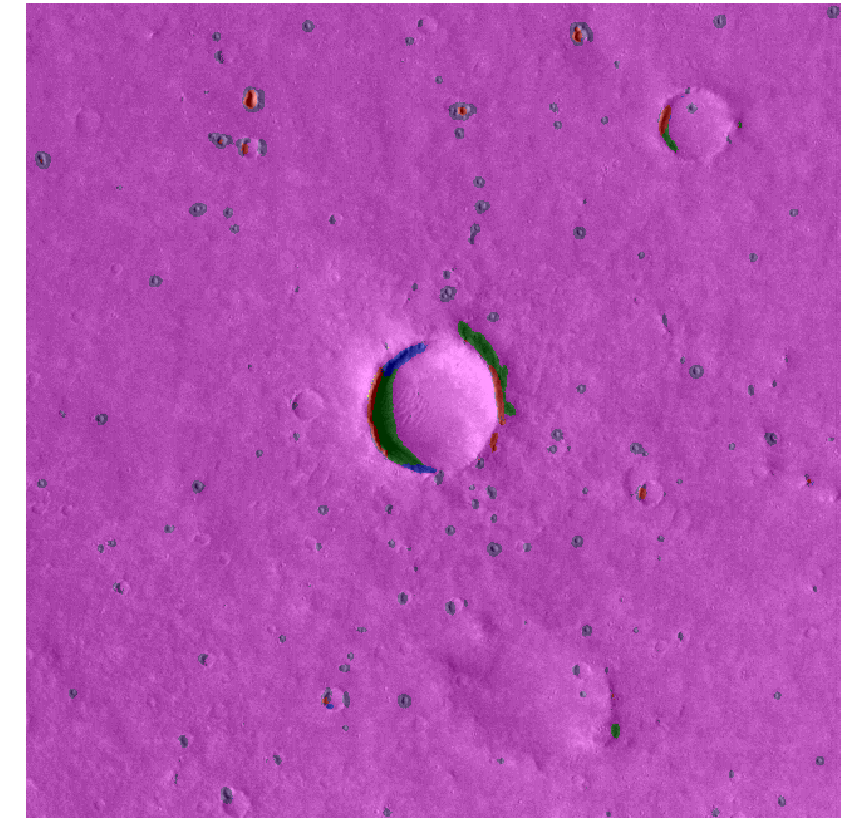
\includegraphics[width=0.15\textwidth]{images/gen/convolution_number/p03_01.png_3.png} &
		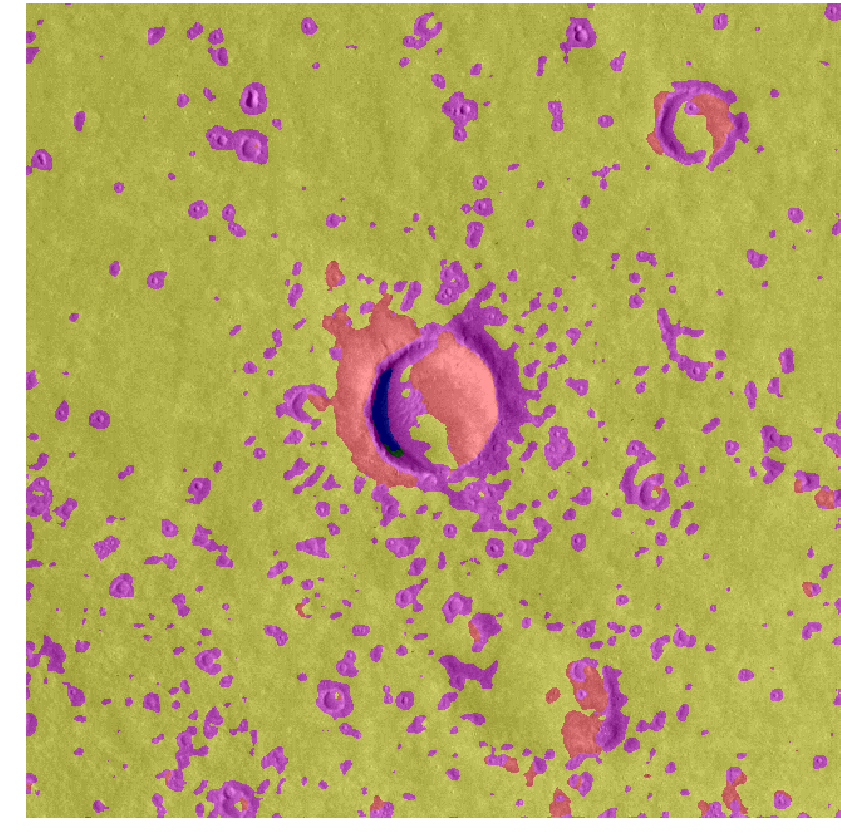
\includegraphics[width=0.15\textwidth]{images/gen/convolution_number/p03_01.png_4.png} &
		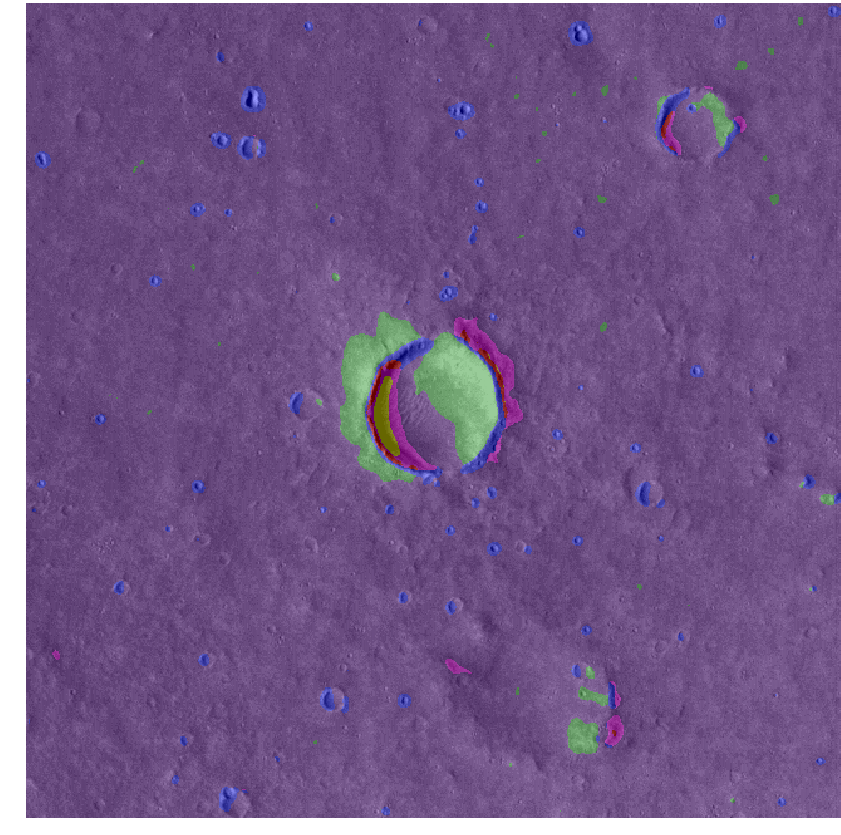
\includegraphics[width=0.15\textwidth]{images/gen/convolution_number/p03_01.png_5.png} &
		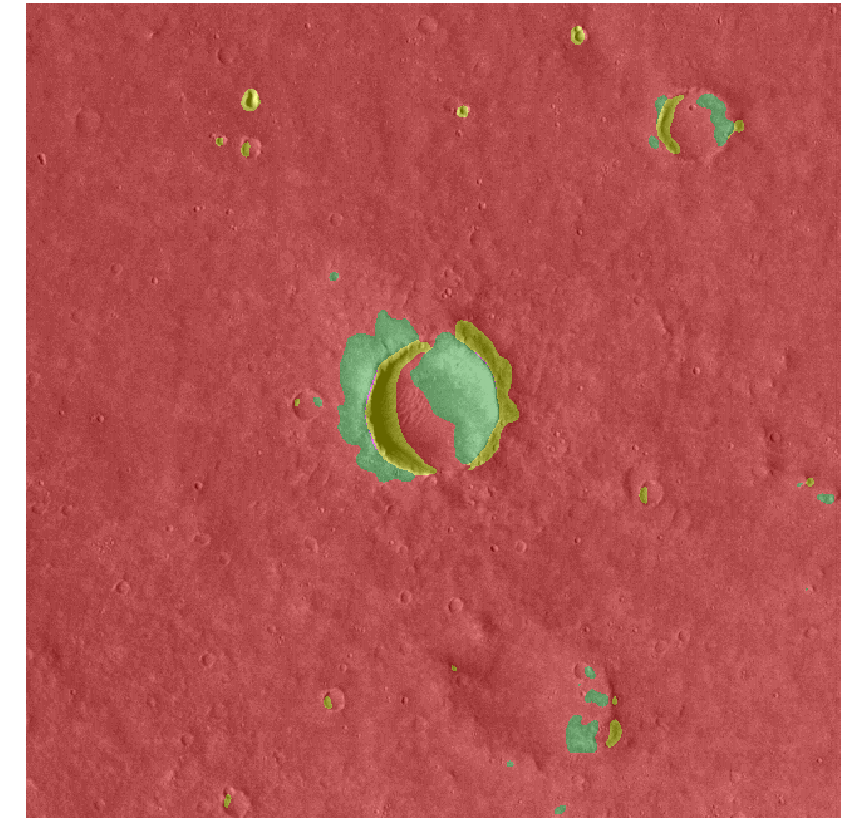
\includegraphics[width=0.15\textwidth]{images/gen/convolution_number/p03_01.png_6.png} \\
		\texttt{b)} &
		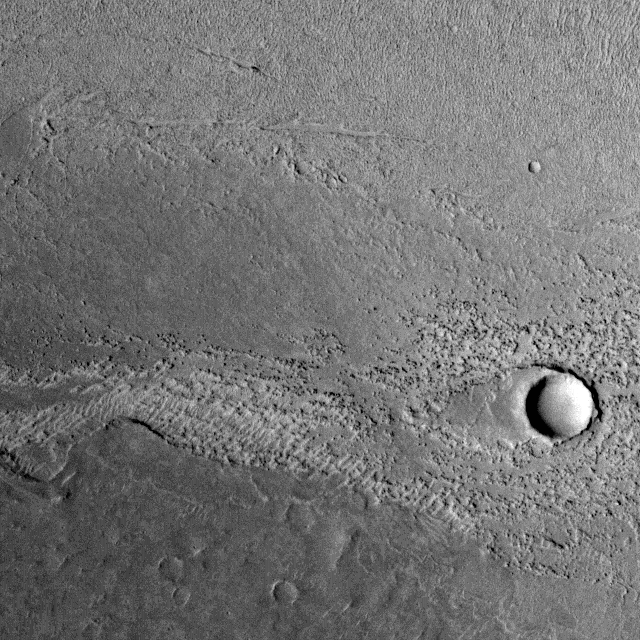
\includegraphics[width=0.15\textwidth]{images/p03/p03_02.png} &
		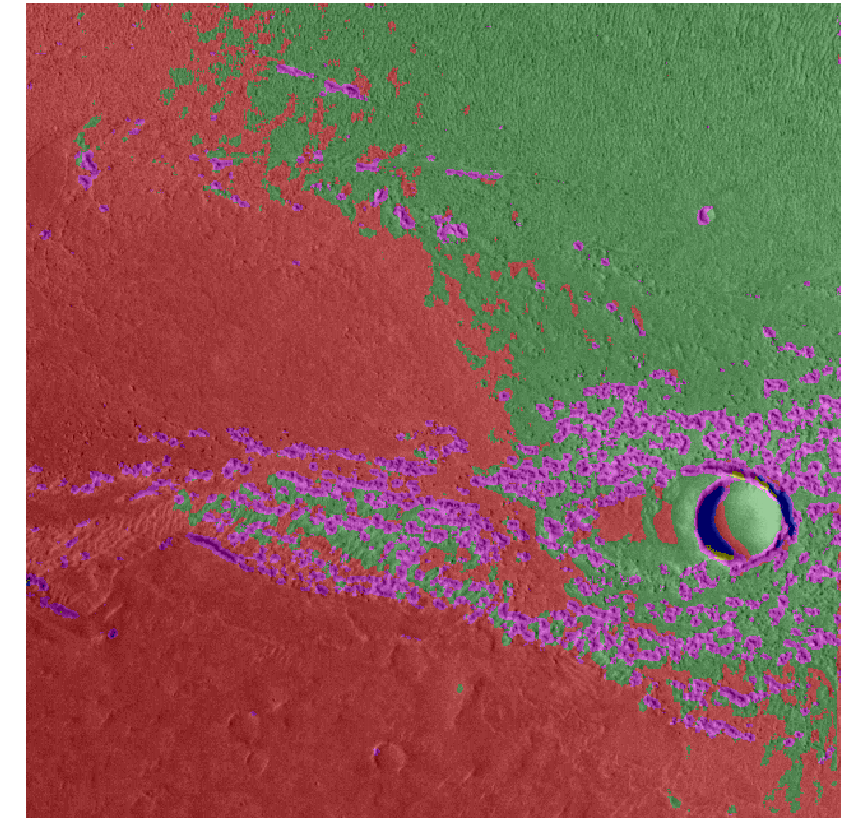
\includegraphics[width=0.15\textwidth]{images/gen/convolution_number/p03_02.png_2.png} &
		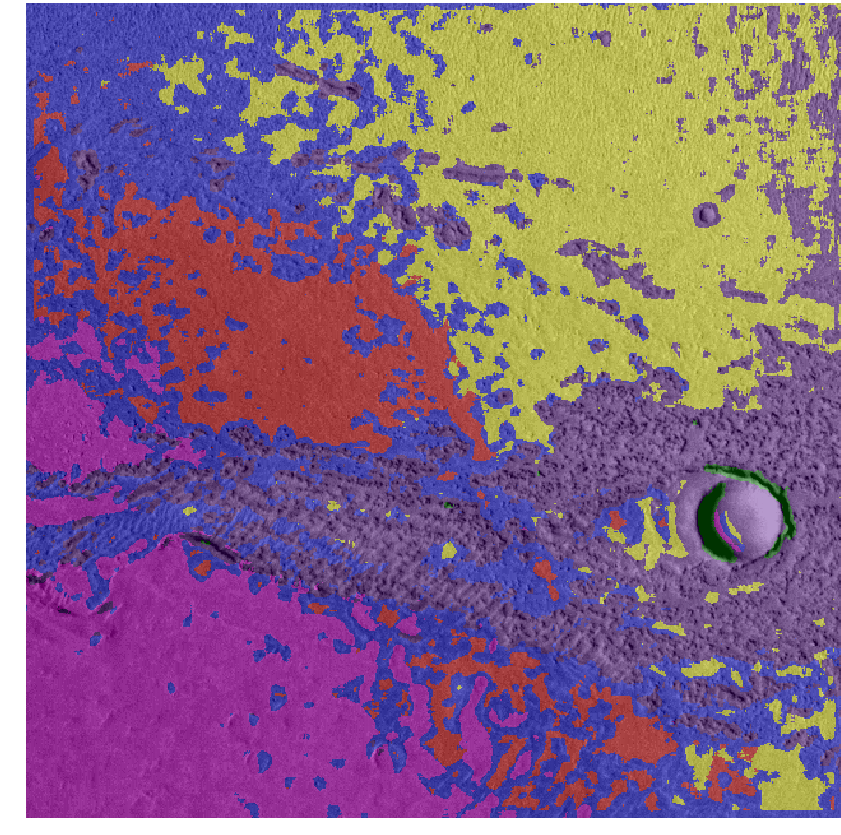
\includegraphics[width=0.15\textwidth]{images/gen/convolution_number/p03_02.png_3.png} &
		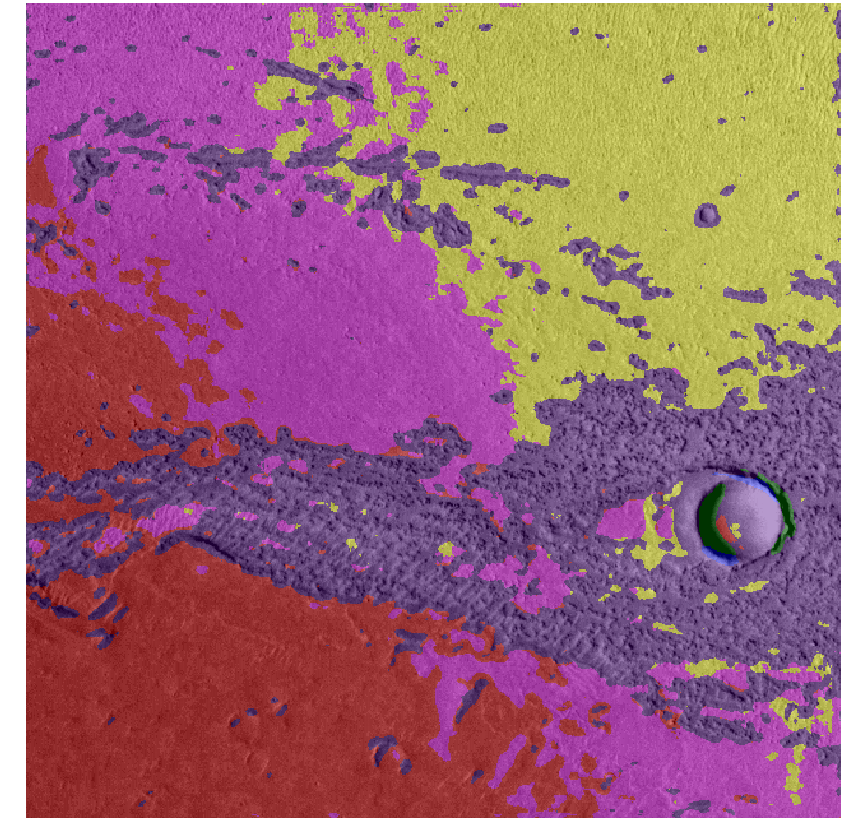
\includegraphics[width=0.15\textwidth]{images/gen/convolution_number/p03_02.png_4.png} &
		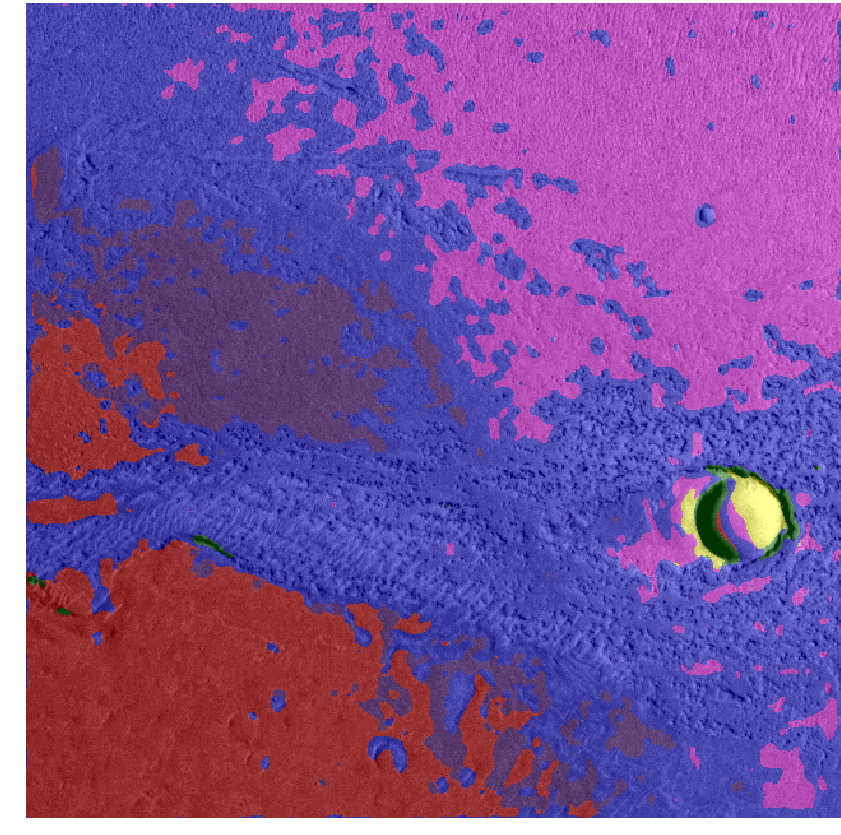
\includegraphics[width=0.15\textwidth]{images/gen/convolution_number/p03_02.png_5.png} &
		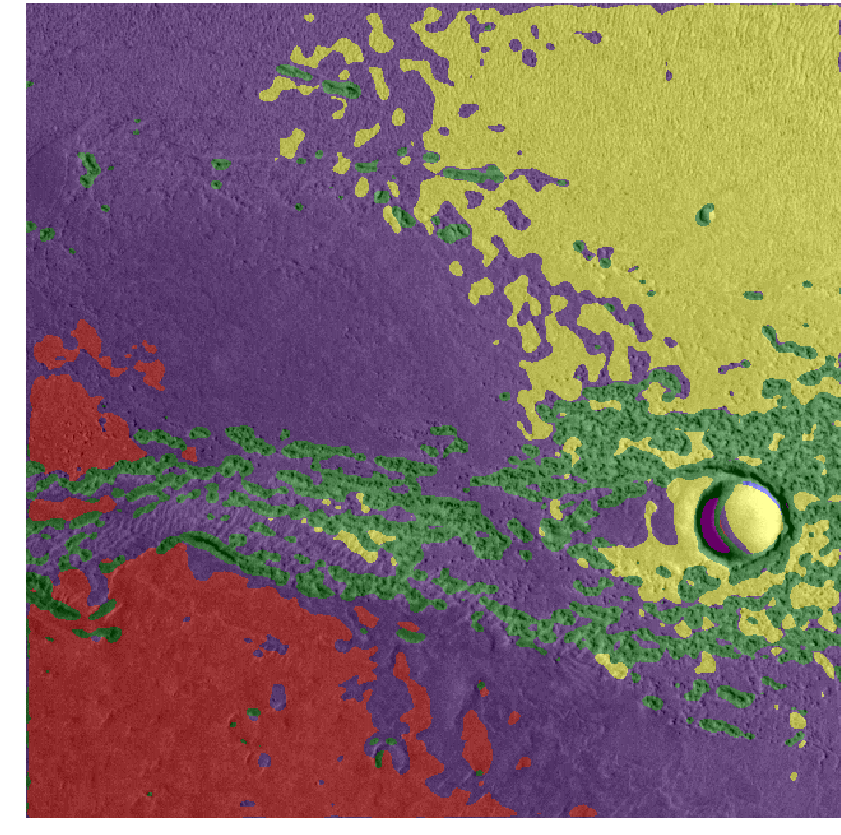
\includegraphics[width=0.15\textwidth]{images/gen/convolution_number/p03_02.png_6.png} \\
		\texttt{c)} &
		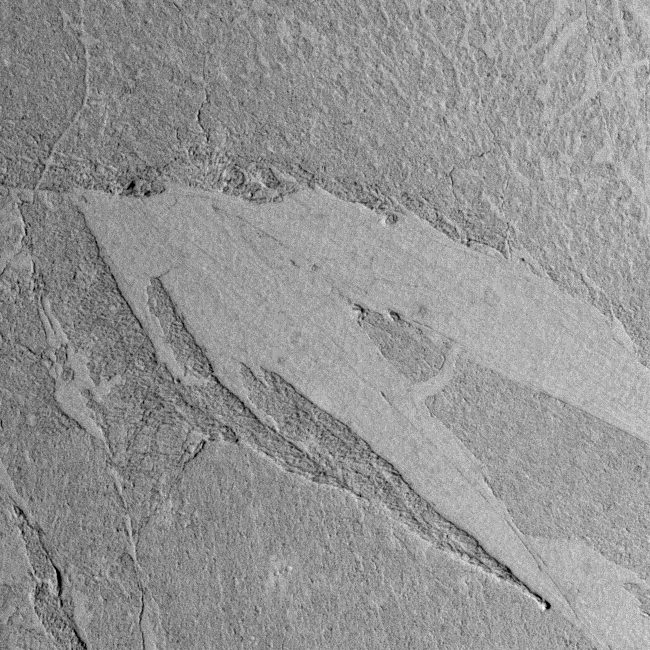
\includegraphics[width=0.15\textwidth]{images/p03/p03_03.png} &
		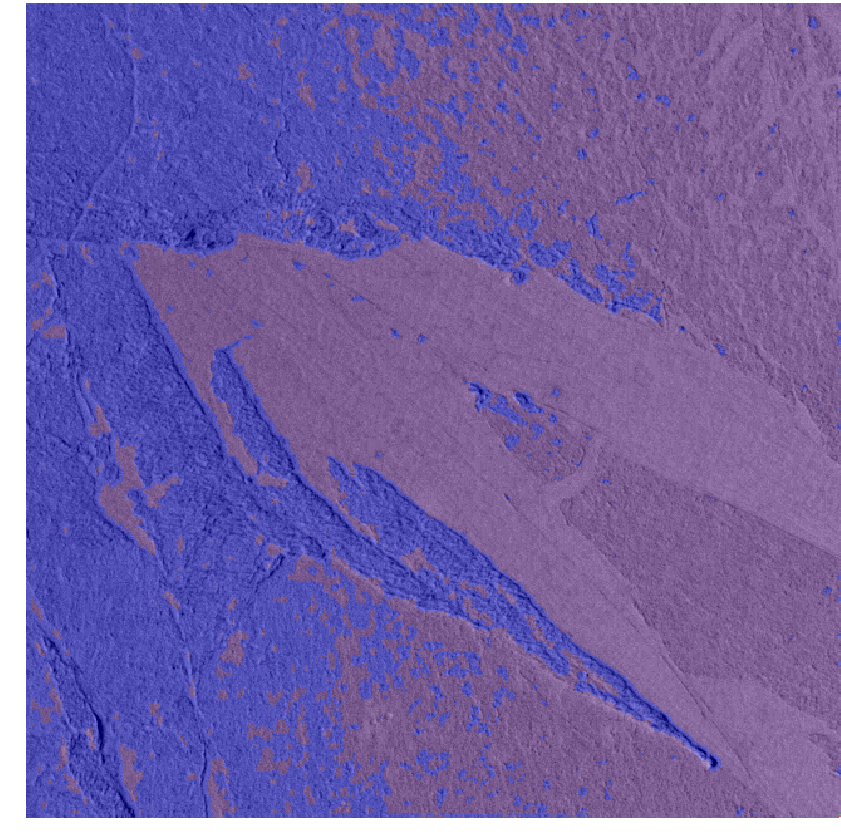
\includegraphics[width=0.15\textwidth]{images/gen/convolution_number/p03_03.png_2.png} &
		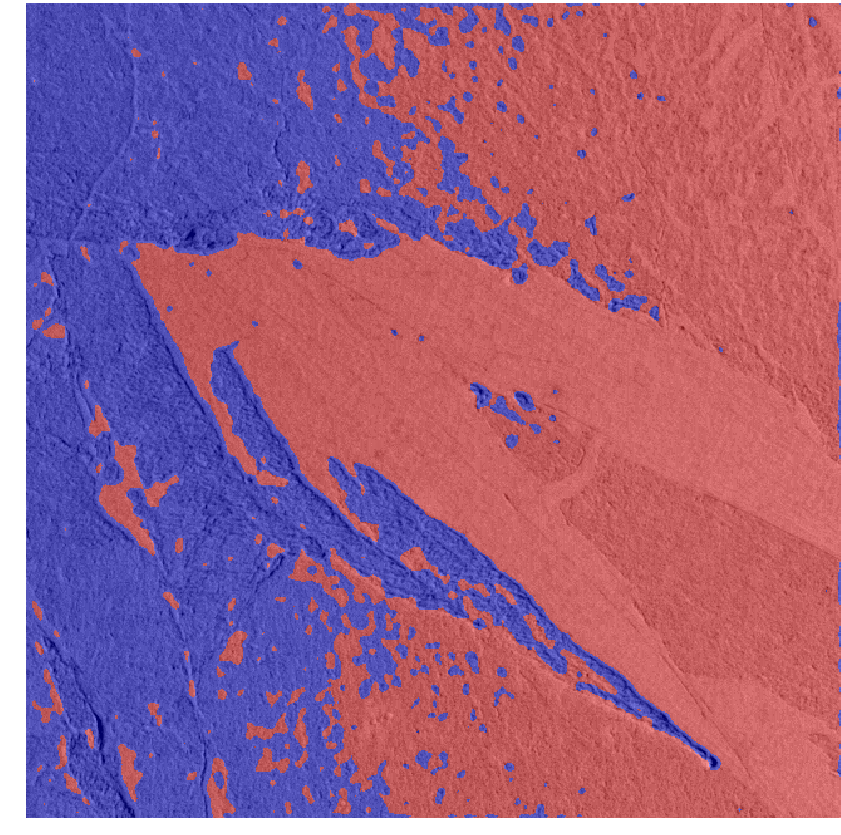
\includegraphics[width=0.15\textwidth]{images/gen/convolution_number/p03_03.png_3.png} &
		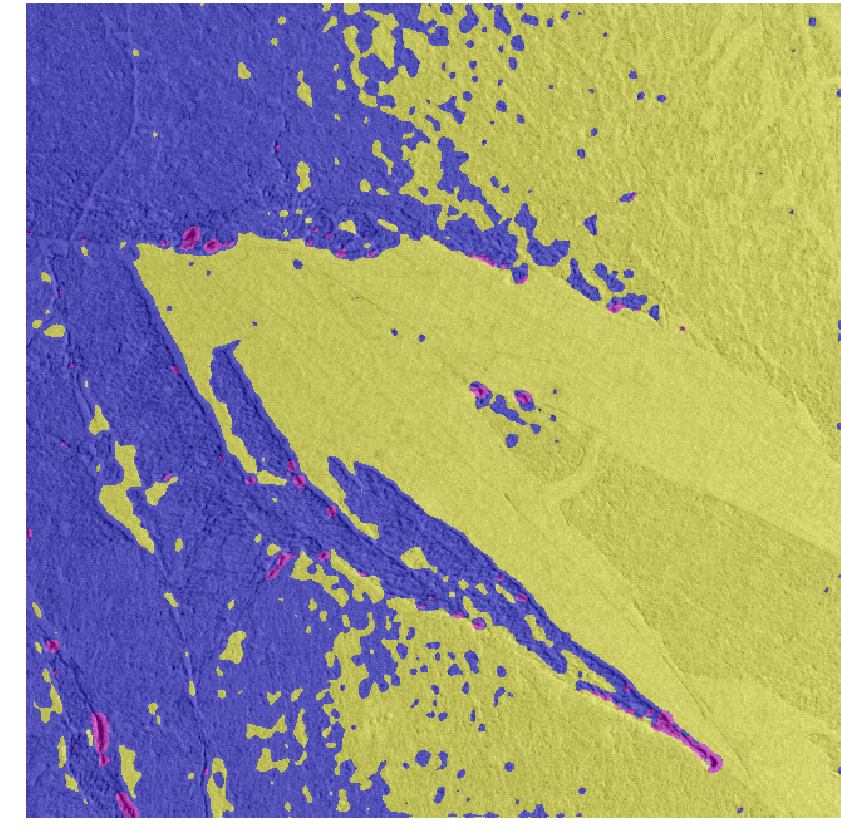
\includegraphics[width=0.15\textwidth]{images/gen/convolution_number/p03_03.png_4.png} &
		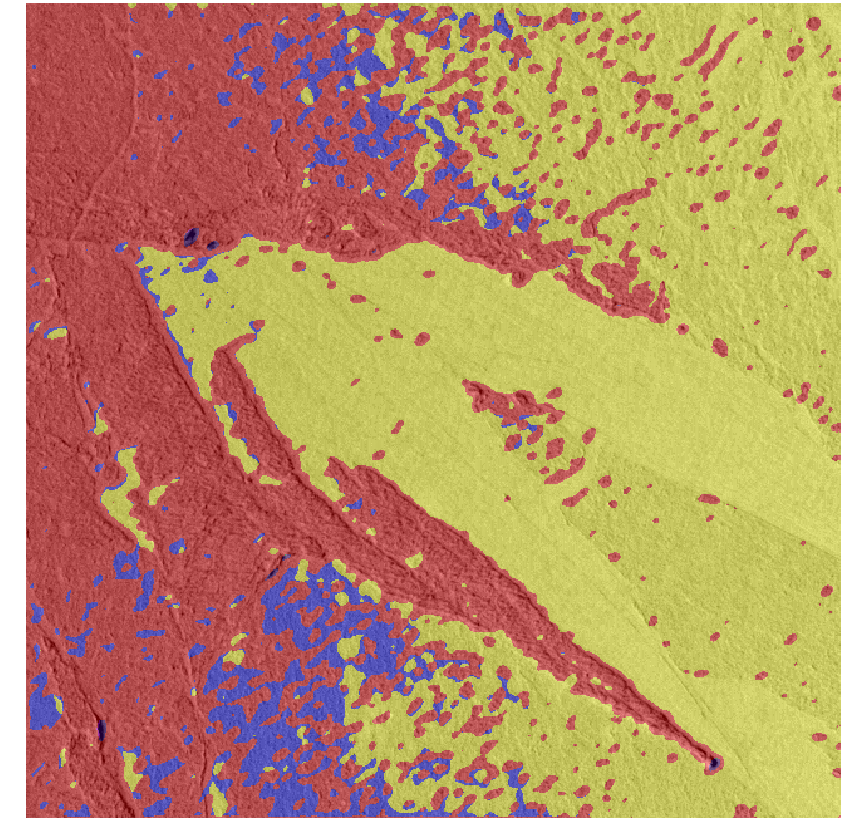
\includegraphics[width=0.15\textwidth]{images/gen/convolution_number/p03_03.png_5.png} &
		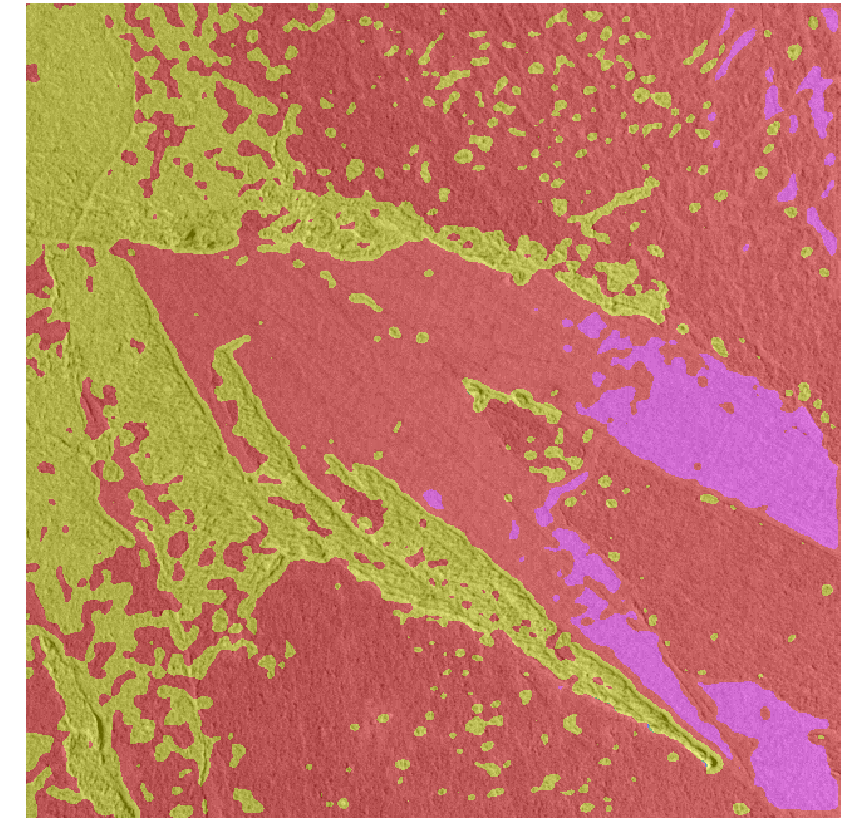
\includegraphics[width=0.15\textwidth]{images/gen/convolution_number/p03_03.png_6.png} \\
		\texttt{d)} &
		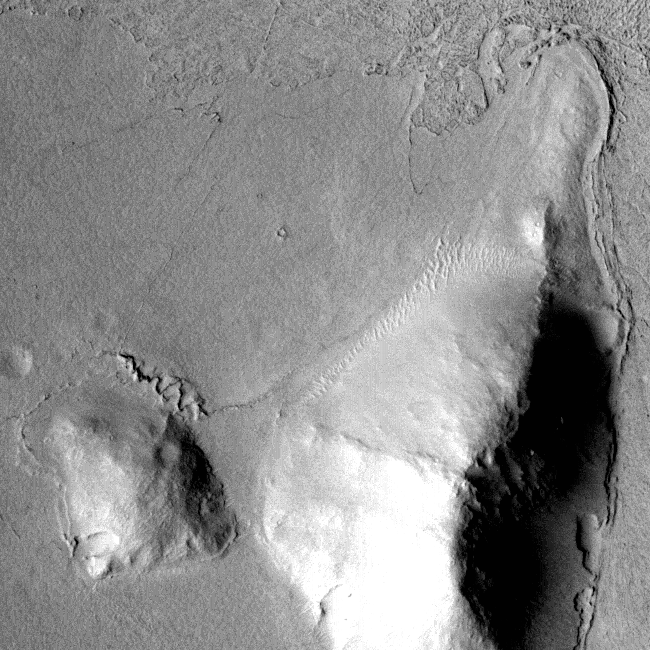
\includegraphics[width=0.15\textwidth]{images/p03/p03_04.png} &
		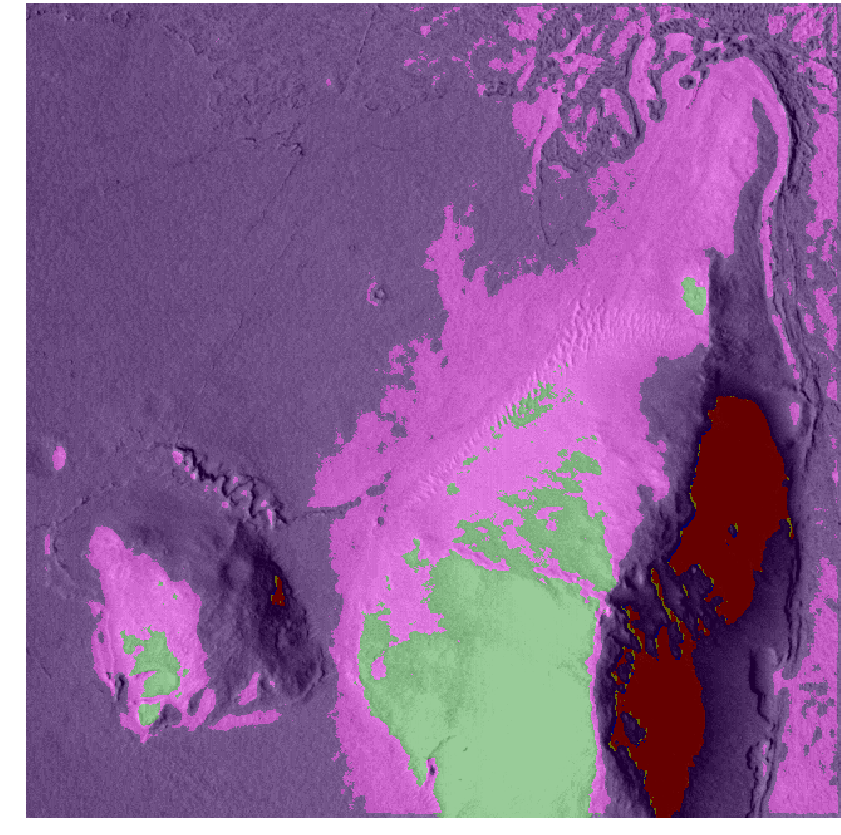
\includegraphics[width=0.15\textwidth]{images/gen/convolution_number/p03_04.png_2.png} &
		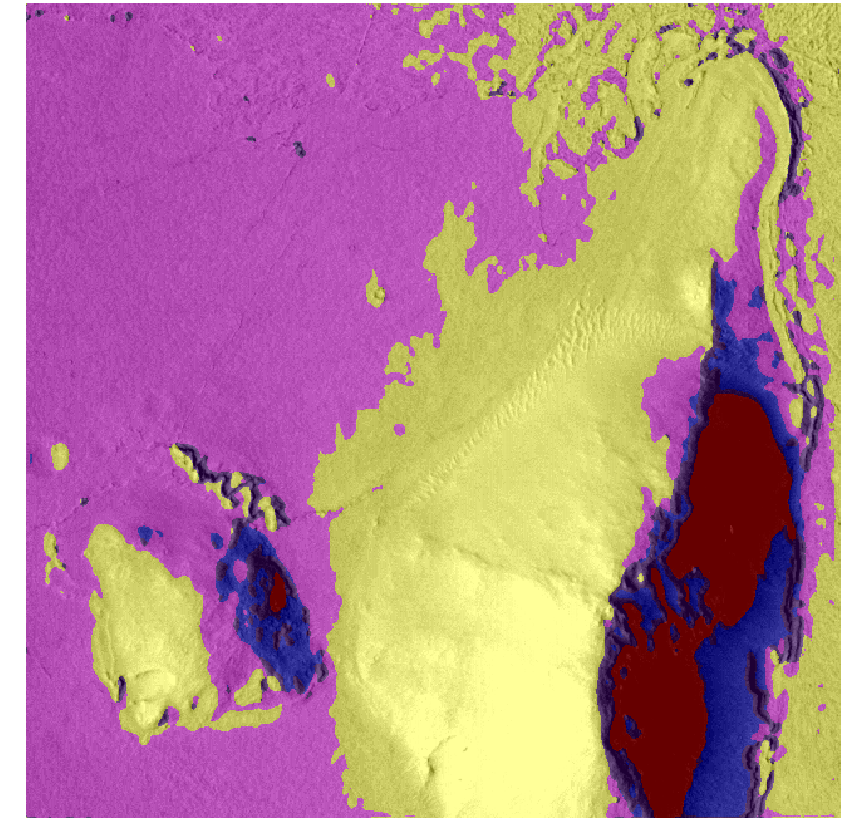
\includegraphics[width=0.15\textwidth]{images/gen/convolution_number/p03_04.png_3.png} &
		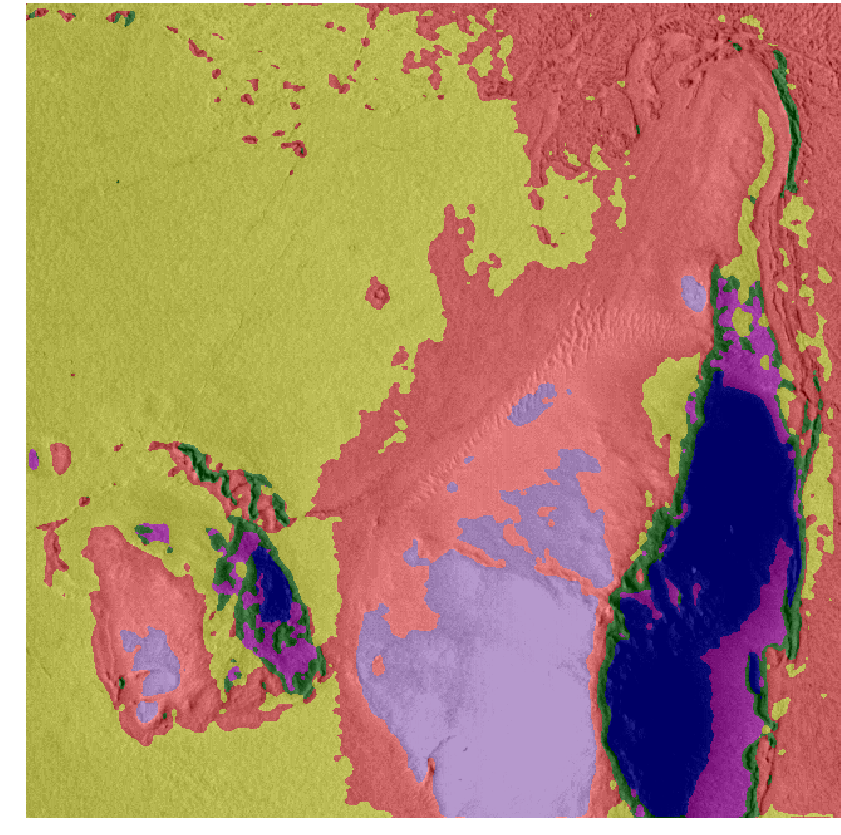
\includegraphics[width=0.15\textwidth]{images/gen/convolution_number/p03_04.png_4.png} &
		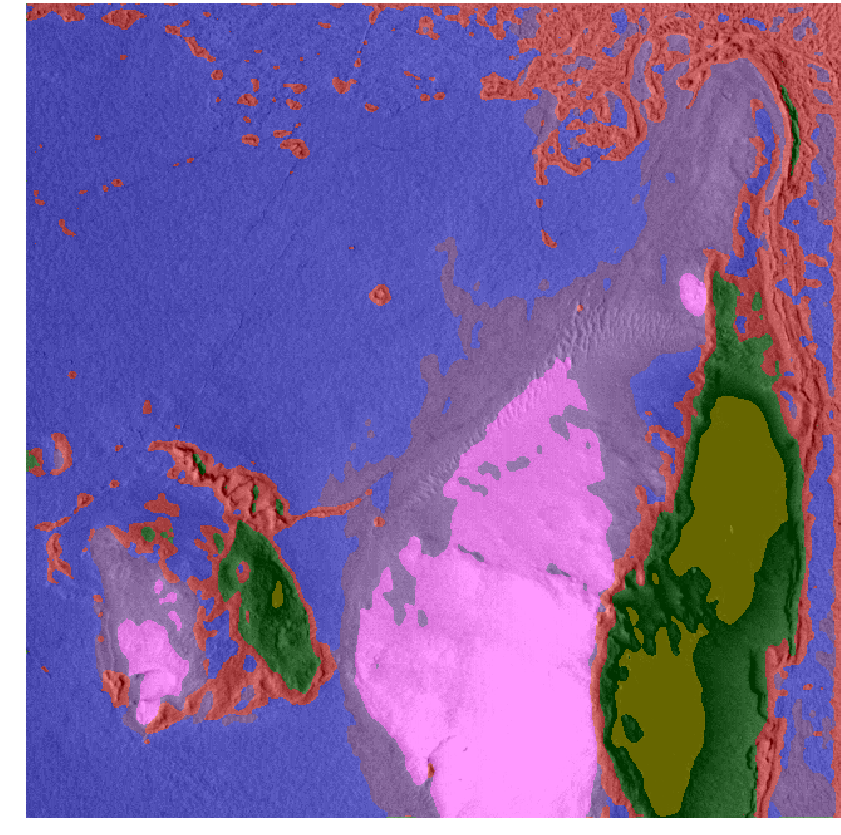
\includegraphics[width=0.15\textwidth]{images/gen/convolution_number/p03_04.png_5.png} &
		\includegraphics[width=0.15\textwidth]{images/gen/convolution_number/p03_04.png_6.png} \\
		
		&
		\vspace*{2pt}\centering Eingabe & 
		\vspace*{2pt}\centering $n_{conv}=2$ &
		\vspace*{2pt}\centering $n_{conv}=3$ &
		\vspace*{2pt}\centering $n_{conv}=4$ &
		\vspace*{2pt}\centering $n_{conv}=5$ &
		\vspace*{2pt}\centering $n_{conv}=6$ 
	\end{tabular}
	\caption{Vergleich der Auswirkungen der Änderung der Anzahl an Konvolutionsschichten. Die Farben der jeweiligen Cluster wurden zufällig gewählt.}
	\label{fig:n_layers_comparision}
\end{figure}

Insgesamt fällt hier kein signifikanter Unterschied zwischen den einzelnen Aufnahmen auf: Ein Großteil der Verbesserungen und Verschlechterungen bei der Modifikation der Anzahl der Konvolutionsschichten ist schlichtweg auf die unterschiedliche Initialisierung des texturbasierten Clusterings und des Netzwerkes selbst zurückzuführen. Erkennbar ist dies daran, dass in der zweiten Aufnahme, bei fünf Konvolutionsschichten eine vergleichbar schlechte Segmentierung generiert wird, diese wird allerdings wieder besser, egal ob eine Konvolutionsschicht hinzugefügt oder entfernt wird.

In Aufnahme \texttt{c)} verändert sich die Segmentierung zwischen $n_{conv}=2$ und $n_{conv}=5$ kaum, lediglich bei $n_{conv}=6$ wird der rechte Bereich als ein weiteres Segment erkannt. Dieser Effekt erschien über mehrere Ausführen des Experimentes hinweg auch nicht zuverlässig, es ist daher auch nur mit einer unterschiedlichen Initialisierung begründet.

\iffalse
\subsection{Größe des Konvolutionskernels}
\subsection{Learning Rate}


%\section{Preprocessing}
%\label{sec:preprocessing}
\fi
\section{Anpassungen zur Segmentierung von mehrfarbigen Fotografien}
\label{sec:color_picture_optimization}

Mehrfarbige Eingabedateien besitzen mehr Merkmale, welche zur Analyse genutzt werden können, da sie zusätzlich Informationen über den Rot, Grün-, und Blauwert der einzelnen Pixel enthalten. Außerdem sind die Motive allgemeiner Fotografieren (wie \zB die des BSDS500-Datensatzes, \vgl Unterabschnitt~\ref{ssec:bsds500}) unterschiedlich zu denen, die bisher genutzt wurden.
Aus diesen Ursachen eignen sich die bisher genannten Parameter nicht universell sowohl zur Segmentierung einer Aufnahme der Marsoberfläche, als auch zur Segmentierung \enquote{normaler} Fotografien.